\section{Synchronizing Bidirectional Transformations}

\mnote{Extend consistency preservation rules to accept models that are not consistent}
In the following, we discuss how we can extend bidirectional transformations and especially their unidirectional consistency preservation rules such that they are able to deal with the situation that both models may have been modified.
To achieve this, we extend consistency preservation rules such that they also accept models that are not initially consistent.
We can then not require them to restore consistency between the models with a single execution anymore.
Instead, we define a notion of \emph{partial consistency}, which allows us to specify how the execution of consistency preservation rules has to improve partial consistency.
We derive requirements to the transformations and finally show that transformations fulfilling these requirements terminate consistently.


\subsection{Partial Consistency of Models}

\mnote{Changed models still fulfill some kind of partial consistency notion}
Given two models $\model{m}{1}$ and $\model{m}{2}$ and changes $\change{\metamodel{M}{1}}$ and $\change{\metamodel{M}{2}}$ to each of them, a unidirectional consistency preservation rule $\consistencypreservationrule{\consistencyrelationset{CR}}^{\rightarrow}$ needs to accept and process the change in one model, be it $\change{\metamodel{M}{1}}$ without loss of generality, and receive the unchanged model $\model{m}{1}$ as well as the changed second model $\change{\metamodel{M}{2}}(\model{m}{2})$.
We discussed the necessity to process the changed second model in the previous section.
Whereas $\model{m}{1}$ and $\model{m}{2}$ are consistent, $\model{m}{1}$ and $\change{\metamodel{M}{2}}(\model{m}{2})$ may not.
In consequence, $\consistencypreservationrule{\consistencyrelationset{CR}}^{\rightarrow}$, even if correct according to \autoref{def:unidirectionalconsistencypreservationrulecorrectness}, cannot guarantee that applying the delivered change delivers consistent models.
$\model{m}{1}$ and $\change{\metamodel{M}{2}}(\model{m}{2})$ will, however, usually still fulfill some kind of partial consistency notion.
Depending on the complexity of $\change{\metamodel{M}{2}}$ large parts of the models will still fulfill some kind of consistency notion.

\mnote{Two options to define partial consistency}
Such a notion of partial consistency may be defined in two different ways.
First, we may say that two models only fulfill the consistency relations partially.
Second, we may say that only extracts of two models fulfill the consistency relations.

\mnote{Partial consistency as fulfilling subsets of consistency relations}
In the first option, we consider that the given models are only consistent to a subset of the given consistency relations.
There may, however, be only a single element in the models that leads to the violation of all consistency relations.
Thus, we would call the models completely inconsistent just because of a single element.
To circumvent hat, we would need to define a notion of partial consistency relations, which allows us to define that models are consistent to parts of consistency relations.
Such a notion would have to be defined at the level of consistency relation pairs and their condition elements within the consistency relations.
It would, however, not make sense to consider subsets of consistency relations, i.e., only a subset of their consistency relation pairs, because when analyzing consistency of two models those consistency relation pairs are not independent.
If two models contain the condition elements of one consistency relation pair, this may prevent the, from containing the condition elements of another consistency relation pair, because in \autoref{def:consistency} we require a unique mapping between condition elements in terms of witness structure.
If models are consistent to a consistency relation in which we removed one (or more) consistency relation pairs, this does not give any reasonable indication on how the models violate consistency.
This may be due to the reason that an element is missing in the models or that an additional element prevents from finding a witness structure.
It does, however, not mean that adding a missing element or removing the additional element ensures that a proper witness structure can be found, because these elements may still be relevant for other consistency relation pairs in the witness structure.
These interdependencies of consistency relation pairs are the reason why consistency to partial consistency relations does not provide insights on the reasons for models being inconsistent.
Thus, we do not consider this as our notion for partial consistency.

\mnote{Partial consistency as parts of the models fulfilling consistency relations}
In the second option, we consider that only parts of the given models are consistent to all given consistency relations.
In addition to the missing ability of the first option to give reasonable insights on inconsistencies, this, intuitively, is a more reasonable notion, because it explicitly defines that parts of the models are consistent, whereas other parts of them are not.
We thus define partial consistency as models having subsets that are actually consistent.
To identify how far models are partially consistent, we also define an according metric.
It is based on the idea to find maximal subsets of the models that are consistent.

\begin{definition}[Partial Consistency] \label{def:partialconsistency}
    Let $\consistencyrelationset{CR}$ be a set of consistency relations.

    Given two models $\model{m}{1} \in \metamodelinstanceset{M}{1}$ and $\model{m}{2} \in \metamodelinstanceset{M}{2}$, we define their \emph{maximal consistent subsets} $\model{m}{1}^p \in \metamodelinstanceset{M}{1}$ and $\model{m}{2}^p \in \metamodelinstanceset{M}{2}$ with regards to $\consistencyrelationset{CR}$ as the subsets of $\model{m}{1}$ and $\model{m}{2}$ that are consistent and larger than all other consistent subsets:
    \begin{align*}
        & 
        \tupled{\model{m}{1}^p, \model{m}{2}^p} \consistenttomath \consistencyrelationset{CR} \land
        \model{m}{1}^p \subseteq \model{m}{1} \land \model{m}{2}^p \subseteq \model{m}{2}  \\
        & \formulaskip
        \land \forall \model{m}{1}^{p'} \in \metamodelinstanceset{M}{1}, \model{m}{2}^{p'} \in \metamodelinstanceset{M}{2} : \\
        & \formulaskip\formulaskip
        \bigl(\model{m}{1}^{p'} \subseteq \model{m}{1} \land \model{m}{2}^{p'} \subseteq \model{m}{2} 
        \land \tupled{\model{m}{1}^{p'}, \model{m}{2}^{p'}} \consistenttomath \consistencyrelationset{CR} \\
        & \formulaskip\formulaskip
        \Rightarrow 
        \abs{\model{m}{1}^{p'}} + \abs{\model{m}{2}^{p'}} \leq \abs{\model{m}{1}^{p}} + \abs{\model{m}{2}^{p}} \bigr)
    \end{align*}
    We define partial consistency of two models with respect to $\consistencyrelationset{CR}$ as the ratio between the size of the maximal consistent subsets and the size of the models in $\function{cons}_{\consistencyrelationset{CR}}$:
    \begin{align*}
        \function{cons}_{\consistencyrelationset{CR}}: \; 
        & (\metamodelinstanceset{M}{1}, \metamodelinstanceset{M}{2}) \rightarrow [0,1] \\
        & 
        (\model{m}{1}, \model{m}{2}) \mapsto \frac{\abs{\model{m}{1}^{p}} + \abs{\model{m}{2}^{p}}}{\abs{\model{m}{1}} + \abs{\model{m}{2}}}
    \end{align*}
    % with:
    % \begin{align*}
    %     & 
    %     \exists \model{m}{1}^p \in \metamodelinstanceset{M}{1}, \model{m}{2}^p \in \metamodelinstanceset{M}{2} : \\
    %     & \formulaskip
    %     \tupled{\model{m}{1}^p, \model{m}{2}^p} \consistenttomath \consistencyrelationset{CR} \land
    %     \model{m}{1}^p \subseteq \model{m}{1} \land \model{m}{2}^p \subseteq \model{m}{2} : \\
    %     & \formulaskip
    %     \land \forall \model{m}{1}^{p'} \in \metamodelinstanceset{M}{1}, \model{m}{2}^{p'} \in \metamodelinstanceset{M}{2} : \\
    %     & \formulaskip\formulaskip
    %     \bigl(\model{m}{1}^{p'} \subseteq \model{m}{1} \land \model{m}{2}^{p'} \subseteq \model{m}{2} 
    %     \land \tupled{\model{m}{1}^{p'}, \model{m}{2}^{p'}} \consistenttomath \consistencyrelationset{CR} \\
    %     & \formulaskip\formulaskip
    %     \Rightarrow 
    %     \abs{\model{m}{1}^{p'}} + \abs{\model{m}{2}^{p'}} \leq \abs{\model{m}{1}^{p}} + \abs{\model{m}{2}^{p}} \bigr) \\
    %     &\formulaskip
    %     \land \function{cons}_{\consistencyrelationset{CR}}(\model{m}{1}, \model{m}{2}) = \abs{\model{m}{1}^{p}} + \abs{\model{m}{2}^{p}}
    % \end{align*}
\end{definition}

\mnote{Partial consistency can always be calculated}
Such maximal consistent subsets do always exist.
In the extreme case, when models are not consistent in any way, it is $\model{m}{1}^p = \model{m}{2}^p = \emptyset$, because empty models are always consistent by definition.
In that case, partial consistency of the models is $0$, whereas in cases when models are actually consistent the maximal consistent subsets are the models themselves, which is why partial consistency is $1$.

% \paragraph{Partielle Konsistenz}
% Gegeben m1, d2(m2) und d1.
% d1(m1) und d2(m2) sind partiell konsistent, d.h. es gibt Teilmengen d1(m1)p und d2(m2)p, für die alle Konsistenzrelationen erfüllt sind.
% Dies kann für mehrere Teilmengen gelten, wir betrachten die, die zusammen maximal groß sind, d.h. |d1(m1)p| + d2(m2)p| > |d1(m1)p'| + d2(m2)p'| für beliebige andere Teilmenge, die konsistent sind.
% TODO: Metrik definieren für partielle Konsistenz. Dann können nämlich einfach sagen, dass sich die partielle Konsistenz erhöhen muss (indem entweder die Modelle kleiner werden oder die konsistenten Teile größer)


\subsection{Transformations for Partially Consistent Models}
\label{chap:synchronization:bidirectional:transformations}

%\todo{Start section again without discussion the starting case for synchronization, but the general case of having partially consistent models. Then later apply it to the starting case for synchronization. Szenario ist, dass wir zwei Modelle reinkriegen (potentiell inkonsistent) und Änderungen an einem davon. Falls das zweite auch geändert wurde, diskutieren wir später, wie wir das noch reinkriegen (indem wir das Delta auf das zweite Modell anwenden und dann die Ausführung der Rückrichtung darauf anwenden).}

\mnote{Multiple executions of consistency preservation rules to resolve partial inconsistencies}
Before we consider the case that two models have been modified and need to be synchronized, we start with the case that of two initially consistent models one has been changed.
We then extend that scenario to the case when both models have been changed.
We use the notion of partial consistency to define that the given models are initially partially consistent and how this partial consistency improves by executing the bidirectional transformation.
As discussed in \autoref{chap:synchronization:combination:bounds}, it may be necessary to execute the consistency preservation rules multiple times to achieve a consistent state, producing several intermediate changes that generate partially consistent models.

\mnote{Execution steps of transformations apply both consistency preservation rules once}
In the following, we derive the properties a bidirectional transformation has to fulfill to eventually return models that are consistent if applied repeatedly.
They are based on the idea that each execution has to improve partial consistency of the given models.
Since a single consistency preservation rule may not be able to improve partial consistency in every case, we always consider the combination of both preservation rules of a bidirectional transformation and require that property from them.
Therefore, we define the notion of a \emph{bidirectional transformation execution step}, which is composed of a single execution of both unidirectional consistency preservation rules.
%This is necessary, because a single consistency preservation rule may not be able to improve partial consistency, whereas at least one of them should be, thus executing both may always lead to an improvement.
%Consider the case that a change was only performed to $\model{m}{2}$, then $\consistencypreservationrule{\consistencyrelationset{CR}}^{\rightarrow}$ cannot produce any reasonable changes in $\model{m}{2}$ to restore consistency.

\begin{definition}[Bidirectional Transformation Execution Step]
    Let $\transformation{t} = \tupled{\consistencyrelationset{CR}, \consistencypreservationrule{\consistencyrelationset{CR}}^{\rightarrow}, \consistencypreservationrule{\consistencyrelationset{CR}}^{\leftarrow}}$ be a bidirectional transformation for metamodels $\metamodel{M}{1}$ and $\metamodel{M}{2}$.
    An \emph{execution step} $\function{Ex}_{\transformation{t}}^1$ of $\transformation{t}$ is a function:
    \begin{align*}
        \function{Ex}_{\transformation{t}}^1 : \; & (\metamodelinstanceset{M}{1}, \metamodelinstanceset{M}{2}, \changeuniverse{\metamodel{M}{1}}) \rightarrow (\metamodelinstanceset{M}{1}, \metamodelinstanceset{M}{2}, \changeuniverse{\metamodel{M}{1}}) \cup \setted{\bot} \\
        & (\model{m}{1}, \model{m}{2}, \change{\metamodel{M}{1}}) \mapsto 
        \begin{cases} 
            (\model{m}{1}', \model{m}{2}', \change{\metamodel{M}{1}}') \\
            \bot
        \end{cases}
    \end{align*}
    with:
    \begin{align*}
        & \change{\metamodel{M}{2}}' = \consistencypreservationrule{\consistencyrelationset{CR}}^{\rightarrow}(\model{m}{1}, \model{m}{2}, \change{\metamodel{M}{1}}) %\\
        & \model{m}{1}' = \change{\metamodel{M}{1}}(\model{m}{1}) \\
        & \change{\metamodel{M}{1}}' = \consistencypreservationrule{\consistencyrelationset{CR}}^{\leftarrow}(\model{m}{2}, \model{m}{1}', \change{\metamodel{M}{2}}') %\\
        & \model{m}{2}' = \change{\metamodel{M}{2}}'(\model{m}{2})
    \end{align*}
    If either consistency preservation rule is undefined for the input, i.e., $\consistencypreservationrule{\consistencyrelationset{CR}}^{\rightarrow}(\model{m}{1}, \model{m}{2}, \change{\metamodel{M}{1}}) = \bot$ or $\consistencypreservationrule{\consistencyrelationset{CR}}^{\leftarrow}(\model{m}{2}, \model{m}{1}', \change{\metamodel{M}{2}}') \bot$, then the execution is undefined, i.e., $\function{Ex}_{\transformation{t}}^1(\model{m}{1}, \model{m}{2}, \change{\metamodel{M}{1}}) = \bot$.
    % for given models $\model{m}{1} \in \metamodelinstanceset{M}{1}$, $\model{m}{2} \in \metamodelinstanceset{M}{2}$ and a change $\change{\metamodel{M}{1}} \in \changeuniverse{\metamodel{M}{1}}$ to $\model{m}{1}$ is the consecutive execution of $\consistencypreservationrule{\consistencyrelationset{CR}}^{\rightarrow}$ and $\consistencypreservationrule{\consistencyrelationset{CR}}^{\leftarrow}}$, i.e.
    % \begin{align*}
    %     & \change{\metamodel{M}{2}}' = \consistencypreservationrule{\consistencyrelationset{CR}}^{\rightarrow}(\model{m}{1}, \model{m}{2}, \change{\metamodel{M}{1}}) \\
    %     & \change{\metamodel{M}{1}}' = \consistencypreservationrule{\consistencyrelationset{CR}}^{\leftarrow}(\model{m}{2}, \change{\metamodel{M}{1}}(\model{m}{1}), \change{\metamodel{M}{2}}')
    % \end{align*}
    % with the resulting changes $\change{\metamodel{M}{1}}'$ and $\change{\metamodel{M}{2}}'$.
\end{definition}

\mnote{Transformation execution steps can be repeatedly applied}
Such execution steps can be applied repeatedly.
Each execution step delivers a new change to the first models and changed versions of the other models by applying the changes delivered by the consistency preservation rules of the bidirectional transformation.
To these resulting models and the resulting change the execution step can be reapplied.
%For models $\model{m}{1} \in \metamodelinstanceset{M}{1}$, $\model{m}{2} \in \metamodelinstanceset{M}{2}$ and a change $\change{\metamodel{M}{1}} \in \changeuniverse{\metamodel{M}{1}}$ to $\model{m}{1}$ and the resulting changes $\change{\metamodel{M}{1}}'$ and $\change{\metamodel{M}{2}}'$ from an execution step, we can apply the next execution step to models $\change{\metamodel{M}{1}}(\model{m}{1})$ and $\change{\metamodel{M}{2}}'(\model{m}{2})$ and the change $\change{\metamodel{M}{1}}'$.

\mnote{Execute transformation by consecutive application of execution steps}
The execution of a bidirectional transformation then consists of the consecutive application of execution steps until the delivered models are consistent, as defined in \autoref{algo:synchronization:executebidirectionaltransformation}.
Although we, theoretically, require the consistency preservation rules to be able to handle initial models that can be arbitrarily inconsistent, it will not be possible to define such rules in practice.
Since we follow a delta-based notion of consistency preservation, we will therefore stick to the requirement that inconsistencies are introduced by changes.
Then it is up to the consistency preservation rules to process the changes in a way and produce new changes that all induced inconsistencies can be resolved.
In contrast to our initial definition of consistency preservation rules, it is still not necessary that consistency is restored with a single execution of a consistency preservation rule.
When finally coming to the synchronization scenario, in which both models have been modified, this will even not be possible anymore.
% \begin{definition}[Bidirectional Transformation Execution]
%     Let $\transformation{t} = \tupled{\consistencyrelationset{CR}, \consistencypreservationrule{\consistencyrelationset{CR}}^{\rightarrow}, \consistencypreservationrule{\consistencyrelationset{CR}}^{\leftarrow}}$ be a bidirectional transformation for metamodels $\metamodel{M}{1}$ and $\metamodel{M}{2}$.
%     An \emph{execution} $\function{Ex}_{\transformation{t}}$ of $\transformation{t}$ is a function
%     \begin{align*}
%         \function{Ex}_{\transformation{t}} : (\metamodelinstanceset{M}{1}, \metamodelinstanceset{M}{2}, \changeuniverse{\metamodel{M}{1}}) \rightarrow (\metamodelinstanceset{M}{1}, \metamodelinstanceset{M}{2}) \cup \setted{\bot}
%     \end{align*}
%     which consecutively applies the execution steps until a consistent pair of models is reached, i.e.:
%     \begin{align*}
%         & 
%         \forall \model{m}{1} \in \metamodelinstanceset{M}{1}, \model{m}{2} \in \metamodelinstanceset{M}{2}, \change{\metamodel{M}{1}} \in \changeuniverse{\metamodel{M}{1}}:  \\
%         & \formulaskip
%         \bigl(\exists \model{m}{1}' \in \metamodelinstanceset{M}{1}, \model{m}{2}' \in \metamodelinstanceset{M}{2}, \change{\metamodel{M}{1}}' \in \changeuniverse{\metamodel{M}{1}}, i \in \mathbb{N} : \\
%         & \formulaskip\formulaskip
%         (\function{Ex}_{\transformation{t}}^1)^i(\model{m}{1}, \model{m}{2}, \change{\metamodel{M}{1}}) = (\model{m}{1}', \model{m}{2}', \change{\metamodel{M}{1}}') \\
%         & \formulaskip\formulaskip
%         \land \tupled{\change{\metamodel{M}{1}}(\model{m}{1}'), \model{m}{2}'} \consistenttomath \consistencyrelationset{CR} \big) \\
%         & \formulaskip\formulaskip\formulaskip
%         \Rightarrow \function{Ex}_{\transformation{t}}(\model{m}{1}, \model{m}{2}, \change{\metamodel{M}{1}}) = (\change{\metamodel{M}{1}}(\model{m}{1}'), \model{m}{2}')
%     \end{align*}
%     % \begin{align*}
%     %     & 
%     %     \forall \model{m}{1} \in \metamodelinstanceset{M}{1}, \model{m}{2} \in \metamodelinstanceset{M}{2}, \change{\metamodel{M}{1}} \in \changeuniverse{\metamodel{M}{1}}: \function{Ex}_{\transformation{t}}(\model{m}{1}, \model{m}{2}, \change{\metamodel{M}{1}}) = \bot \\
%     %     & \formulaskip
%     %     \lor \big(\exists \model{m}{1}' \in \metamodelinstanceset{M}{1}, \model{m}{2}' \in \metamodelinstanceset{M}{2}, \change{\metamodel{M}{1}}' \in \changeuniverse{\metamodel{M}{1}}, i \in \mathbb{N} : \\
%     %     & \formulaskip\formulaskip
%     %     (\function{Ex}_{\transformation{t}}^1)^i(\model{m}{1}, \model{m}{2}, \change{\metamodel{M}{1}}) = (\model{m}{1}', \model{m}{2}', \change{\metamodel{M}{1}}') \\
%     %     & \formulaskip\formulaskip
%     %     \land \function{Ex}_{\transformation{t}}(\model{m}{1}, \model{m}{2}, \change{\metamodel{M}{1}}) = (\change{\metamodel{M}{1}}(\model{m}{1}'), \model{m}{2}') \\
%     %     & \formulaskip\formulaskip
%     %     \land \tupled{\change{\metamodel{M}{1}}(\model{m}{1}'), \model{m}{2}'} \consistenttomath \consistencyrelationset{CR} \big)
%     % \end{align*}
%     % for given models $\model{m}{1} \in \metamodelinstanceset{M}{1}$, $\model{m}{2} \in \metamodelinstanceset{M}{2}$ and a change $\change{\metamodel{M}{1}} \in \changeuniverse{\metamodel{M}{1}}$ to $\model{m}{1}$ is the consecutive application of execution steps, i.e.
%     % \begin{align*}
%     %     \func{Ex}_{\transformation{t}} : & (\metamodelinstanceset{M}{1}, \metamodelinstanceset{M}{2}, \changeuniverse{\metamodel{M}{1}) \rightarrow (\metamodelinstanceset{M}{1}, \metamodelinstanceset{M}{2}) \\
%     %     & (\model{m}{1}, \model{m}{2}, \change{\metamodel{M}{1}) \mapsto 
%     %         \begin{cases} 
%     %             (\model{m}{1}', \model{m}{2}'), \exists i \in \mathbb{N} : \func{Ex}_{\transformation{t}}^i(\model{m}{1}, \model{m}{2}, \change{\metamodel{M}{1}) = (\model{m}{1}'', \model{m}{2}', \change{\metamodel{M}{1}') \land \model{m}{1}' = \change{\metamodel{M}{1}'(\model{m}{1}'') \land \tupled{\model{m}{1}', \model{m}{2}'} \consistenttomath \consistencyrelationset{CR} \\
%     %             \bot, otherwise
%     %         \end{cases}
%     %     \end{align*}
% \end{definition}

\begin{algorithm}
    \begin{algorithmic}[1]
    \Procedure{\function{Execute}}{$\transformation{t} = \tupled{\consistencyrelationset{CR}, \consistencypreservationrule{\consistencyrelationset{CR}}^{\rightarrow}, \consistencypreservationrule{\consistencyrelationset{CR}}^{\leftarrow}}, \model{m}{1}, \model{m}{2}, \change{\metamodel{M}{1}}$}
        \algindentskip
        \If{$\neg (\tupled{\model{m}{1}, \model{m}{2}} \consistenttomath \consistencyrelationset{CR})$}
            \State \Return{$\bot$}
        \EndIf
        \algblockskip

        \While{$\neg (\tupled{\change{\metamodel{M}{1}}(\model{m}{1}), \model{m}{2}} \consistenttomath \consistencyrelationset{CR})$}
            \State $(\model{m}{1}, \model{m}{2}, \change{\metamodel{M}{1}}) \gets \function{Ex}_\transformation{t}^1(\model{m}{1}, \model{m}{2}, \change{\metamodel{M}{1}})$
            \If{$(\model{m}{1}, \model{m}{2}, \change{\metamodel{M}{1}}) = \bot$}
                \State \Return{$\bot$} \label{algo:synchronization:execute_bidirectional_transformation:line:returnbot}
            \EndIf
        \EndWhile
        \algblockskip

        \State \Return{$\tupled{\change{\metamodel{M}{1}}(\model{m}{1}), \model{m}{2}}$} \label{algo:synchronization:execute_bidirectional_transformation:line:returnresult}
        \algindentskip
    \EndProcedure
\end{algorithmic}
    \caption[Execution of a bidirectional transformation]{Execution of a bidirectional transformation.}
    \label{algo:synchronization:executebidirectionaltransformation}
\end{algorithm}

\todo{Möglicherweise müssen wir hier auch noch die Deltas rausgeben, weil die ja von den anderen Transformationen im Netzwerk noch bearbeitet werden müssen. Hierfür könnten wir später definieren, wann eine BX Sync emulierend ist.}

%\todo{Discuss how to realize that function in an algorithm}

\mnote{Execution step can be defined for changes to either of the models}
Without loss of generality, we defined bidirectional transformation execution and the individual execution steps for original changes in $\metamodel{M}{1}$, although the consistency preservation rules of a transformation are also able to handle changes in $\metamodel{M}{2}$.
The definitions can be applied to that case accordingly, just by swapping $\consistencypreservationrule{\consistencyrelationset{CR}}^{\rightarrow}$ and $\consistencypreservationrule{\consistencyrelationset{CR}}^{\leftarrow}$.
Since we finally consider the case that both models have been changed, it is not relevant for us which change to consider first anyway.

%\todo{Reihenfolge diskutieren: o.B.d.A. haben wir eine Reihenfolge verwendet, aber es müssen natürlich beide gehen, da in jedem Modell Änderungen passieren können. Wenn beide Modelle geändert sind (wo wir hinwollen), ist es im Prinzip wieder egal. Aber in der Praxis kann es schon einen Unterschied machen, weil eine Richtung sinnvollerweise zuerst ausgeführt wird.
%Das meiste hiervon ist im vorigen Absatz adressiert, aber später wenn wir das Synchronisationszenario diskutieren müssen wir nochmal darauf eingehen, welche Richtung wir zuerst betrachten und welche "reingemergt" wird.}


\subsection{Transformation Execution Termination}

\mnote{Transformation execution either returns $\bot$ or consistent models}
It is obvious that the algorithm does only return $\bot$ if an execution step of the transformation cannot be applied.
Additionally, we can easily show that in all other cases, if the algorithm terminates, it returns consistent models.

\begin{lemma}{Bidirectional Transformation Execution Consistency}
    \label{lemma:bidirectionaltransformationconsistency}
    If \autoref{algo:synchronization:executebidirectionaltransformation} terminates, it either returns $\bot$ or a consistent model pair.
\end{lemma}
\begin{proof}
    \autoref{algo:synchronization:executebidirectionaltransformation} can terminate by one of its two return statements in \autoref{algo:synchronization:executebidirectionaltransformation:line:returnbot} and \autoref{algo:synchronization:executebidirectionaltransformation:line:returnresult}.
    \autoref{algo:synchronization:executebidirectionaltransformation:line:returnbot} returns $\bot$, which fulfills the lemma statement.
    \autoref{algo:synchronization:executebidirectionaltransformation:line:returnresult} returns the model pair $\tupled{\change{\metamodel{M}{1}}(\model{m}{1}), \model{m}{2}}$.
    The only possibility to achieve this statement is the termination of the previous while loop.
    Since there is no statement to terminate the loop, except for the other return statement and the non-fulfillment of the loop condition, we can only reach this statement by non-fulfillment of the loop condition.
    Since the negation of the loop condition is $\tupled{\change{\metamodel{M}{1}}(\model{m}{1}), \model{m}{2}} \consistenttomath \consistencyrelationset{CR}$, the result fulfills the lemma statement.
\end{proof}

\mnote{Transformation execution does not necessarily terminate}
The algorithm does, however, not ensure termination for arbitrary bidirectional transformations and input models and changes.
To ensure termination, we need to assure that after a finite number of execution steps of the transformation either no further execution step can be applied, i.e., it returns $\bot$, or it delivers consistent models.
To achieve this, we enforce execution steps to improve partial consistency to finally reach a consistent state. 
We provide the following notion of \enquote{partial consistency improvement} for that.

\begin{definition}[Partial-Consistency-Improving Bidirectional Transformation]
    \label{def:partialconsistencyimprovingtransformation}
    Let $\transformation{t} = \tupled{\consistencyrelationset{CR}, \consistencypreservationrule{\consistencyrelationset{CR}}^{\rightarrow}, \consistencypreservationrule{\consistencyrelationset{CR}}^{\leftarrow}}$ be a bidirectional transformation for metamodels $\metamodel{M}{1}$ and $\metamodel{M}{2}$.
    We say that $\transformation{t}$ is \emph{partial-consistency-improving} if, and only if, an execution step does always improve partial consistency by reducing size of the models or improving size of the consistent subsets.
    So for all inputs, for which the execution step of $\transformation{t}$ does not return $\bot$,
    \begin{align*}
        & (\model{m}{1}', \model{m}{2}', \change{\metamodel{M}{1}}') \equalsperdefinition \function{Ex}_{\transformation{t}}^1(\model{m}{1}, \model{m}{2}, \change{\metamodel{M}{1}})
    \end{align*}
    we denote $\change{\metamodel{M}{1}}(\model{m}{1})^p$ and $\model{m}{2}^p$ as the maximal consistent subsets of $\tupled{\change{\metamodel{M}{1}}(\model{m}{1}), \model{m}{2}}$ and $\change{\metamodel{M}{1}}'(\change{\metamodel{M}{1}}(\model{m}{1}))^p$ and $\change{\metamodel{M}{2}}'(\model{m}{2})^p$ as the ones of $\tupled{\change{\metamodel{M}{1}}'(\change{\metamodel{M}{1}}(\model{m}{1})), \change{\metamodel{M}{2}}'(\model{m}{2})}$
    and require that when $\change{\metamodel{M}{1}}(\model{m}{1})^p \neq \change{\metamodel{M}{1}}(\model{m}{1})$ and $\model{m}{2}^p \neq \model{m}{2}$:
    \begin{align*}
        &
        \abs{\change{\metamodel{M}{1}}'(\change{\metamodel{M}{1}}(\model{m}{1}))^p} + \abs{\change{\metamodel{M}{2}}'(\model{m}{2})^p} 
        - \abs{\change{\metamodel{M}{1}}(\model{m}{1})^p} - \abs{\model{m}{2}^p} \\
        & \formulaskip
        > \abs{\change{\metamodel{M}{1}}'(\change{\metamodel{M}{1}}(\model{m}{1}))} + \abs{\change{\metamodel{M}{2}}'(\model{m}{2})} 
        - \abs{\change{\metamodel{M}{1}}(\model{m}{1})} - \abs{\model{m}{2}}
        %\Rightarrow %\function{Cons}_\consistencyrelationset{CR}(\change{\metamodel{M}{1}}(\model{m}{1}), \model{m}{2}) < \function{Cons}_\consistencyrelationset{CR}(\change{\metamodel{M}{1}}'(\model{m}{1}'), \model{m}{2}')
    \end{align*}
\end{definition}

\mnote{Partial consistency improvement defines an intuitive expectation to transformations}
Although the definition may first look like a rather theoretic requirement, it obviously matches an intuitive expectation regarding consistency preservation.
In each execution step of the bidirectional transformation, we expect that no existing consistency is destroyed and that further consistency is introduced.
To this end, we expect either the size of the maximal consistent subsets to improve more than the size of the models or the size of the models to decrease more than the size of the maximal consistent subsets.
This is reasonable because consistency preservation should either add or modify elements such that more elements are consistent or remove elements that are inconsistent because their corresponding elements were removed.
In the first case, the size of the maximal consistent subsets is improved by adding or modifying elements such that they are consistent again.
At the same time, models should not increase in size by the same value as the maximal consistent subsets do, because then elements were added which do either not improve consistency of any already existing element or otherwise violate consistency of some of the existing elements.
We do, however, not want consistency preservation rules to violate consistency for any already consistent element.
In the second case, the size of the models is decreased by removing elements which were not consistent because of the removal of a corresponding element.
At the same time, models should not decrease in size by the same value due to the same reasons as in the first case.
If elements are removed from the models, which were also present in the maximal consistent subsets, elements that were actually consistent are removed, which is undesired.
For these reasons, we consider the requirements in \autoref{def:partialconsistencyimprovingtransformation} to be appropriate for practical transformation definition.
They even represent a weaker notion than what we want to achieve in practice, because the requirement are only based on the sizes of the models and their maximal consistent subsets but not the actual contents.
In practice, the consistent subsets before transformation execution will be a subset of those after transformation execution, although this is not formally required by the definition.

\begin{remark}
    The definition for partial-consistency-improving transformations is based on a notion of partial consistency that considers the \emph{maximal} consistent subsets.
    In practice, the subsets of the models that are to be considered consistent may not necessarily be the maximal ones.
    It is possible that there are larger sets subsets that could be considered consistent, but due to the history of changes other, smaller subsets actually represent the consistent subsets.
    The requirement in the formalization is, however, only necessary to be able to have a unique subset that can be calculate from each model state and make statements about.
    In practice, usually trace models are used to represent which elements are corresponding and thus witness consistency.
    Ensuring that the requirements of partial consistency improvement apply to the consistent subsets induced by that trace model, the previous and following insights are still applicable, as it is only necessary that partial consistency improves with each transformation execution step and finally reaches $1$.
\end{remark}

\mnote{Consecutively improving partial consistency does not necessarily lead to consistent models}
The given notion of partial consistency improvement is stronger than the intuitive notion of just requiring the application of an execution step to improve partial consistency according to the metric in \autoref{def:partialconsistency}.
Although expecting such an improvement does also ensure that the execution steps are strongly monotone regarding partial consistency, it does not ensure that a partial consistency value of $1$ is reached after a finite number of execution steps.
This is due to the possibility of just having an asymptotic approximation of $1$, which can, for example, be achieved by adding consistent elements in each step, which do not affect the existing elements.
Then the size of both the maximal consistent subsets as well as the models themselves increases by the same value, thus partial consistency improves but never reaches $1$.

\begin{lemma}[Termination of Partial-Consistency-Improving Bidirectional Transformation Execution]
    \label{lemma:bidirectionaltransformationtermination}
    Let $\transformation{t} = \tupled{\consistencyrelationset{CR}, \consistencypreservationrule{\consistencyrelationset{CR}}^{\rightarrow}, \consistencypreservationrule{\consistencyrelationset{CR}}^{\leftarrow}}$ be a partial-consistency-improving bidirectional transformation.
    Then \autoref{algo:synchronization:executebidirectionaltransformation} does always terminate.
\end{lemma}
\begin{proof}
    The while loop of the algorithm consecutively applies an execution step of the bidirectional transformation $\transformation{t}$.
    The algorithm terminates when at some point a return statement is executed, thus either an execution step cannot be executed and returns $\bot$, or the loop condition is not fulfilled anymore.
    To quit the loop, the model pair $\tupled{\change{\metamodel{M}{1}}(\model{m}{1}), \model{m}{2}}$ needs to be consistent.
    $\model{m}{1}$, $\model{m}{2}$ and $\change{\metamodel{M}{1}}$ are the results of an execution step of $\transformation{t}$, to which the values $\model{m}{1}$, $\model{m}{2}$ and $\change{\metamodel{M}{1}}$ if the previous iteration were given.
    We know that $\tupled{\change{\metamodel{M}{1}}(\model{m}{1}), \model{m}{2}} \consistenttomath \consistencyrelationset{CR}$ if, and only if, their partial consistency is $1$, i.e., $\function{Cons}_\consistencyrelationset{CR}(\change{\metamodel{M}{1}}(\model{m}{1}), \model{m}{2}) = 1$.
    Partial consistency is $1$ if, any only if, the size of the maximal consistent subsets are equal to the sizes of the models themselves, i.e., when $\abs{\change{\metamodel{M}{1}}(\model{m}{1})^p} + \abs{\model{m}{2}^p} = \abs{\change{\metamodel{M}{1}}(\model{m}{1})} + \abs{\model{m}{2}}$.
    To show that partial consistency reaches $1$, we consider the development of the size differences of the maximal consistent subsets and the models.
    We start with the initial size difference
    \begin{align*}
        \mathvariable{sizeDifference}_0 = \abs{\change{\metamodel{M}{1}}(\model{m}{1})} + \abs{\model{m}{2}} - \abs{\change{\metamodel{M}{1}}(\model{m}{1})^p} + \abs{\model{m}{2}^p}
    \end{align*}
    It is $\mathvariable{sizeDifference} \geq 0$, because the models are always larger than their maximal consistent subsets.
    In the $i$-th iteration of the loop, we start with models $\model{m}{1}''$, $\model{m}{2}''$ and change $\change{\metamodel{M}{1}}''$ and the execution step returns models $\model{m}{1}'''$, $\model{m}{2}'''$ and change $\change{\metamodel{M}{1}}'''$.
    Then we have the size differences before that iteration, i.e., the difference after iteration $i-1$, and after that iteration, as:
    \begin{align*}
        &
        \mathvariable{sizeDifference}_{i-1} = \abs{\change{\metamodel{M}{1}}''(\model{m}{1})''} + \abs{\model{m}{2}''} - \abs{\change{\metamodel{M}{1}}''(\model{m}{1})''^p} + \abs{\model{m}{2}''^p} \\
        &
        \mathvariable{sizeDifference}_{i} = \abs{\change{\metamodel{M}{1}}'''(\model{m}{1})''} + \abs{\model{m}{2}'''} - \abs{\change{\metamodel{M}{1}}'''(\model{m}{1})'''^p} + \abs{\model{m}{2}'''^p}
    \end{align*}
    If we consider the reduction of the size difference in the $i$-th iteration, this is given by:
    \begin{align*}
        & 
        \mathvariable{sizeDifferenceReduction}_{i} = \mathvariable{sizeDifference}_{i} - \mathvariable{sizeDifference}_{i-1} \\
        & 
        = \abs{\change{\metamodel{M}{1}}'''(\model{m}{1})''} + \abs{\model{m}{2}'''} - \abs{\change{\metamodel{M}{1}}'''(\model{m}{1})'''^p} + \abs{\model{m}{2}'''^p} \\
        & \formulaskip
        - (\abs{\change{\metamodel{M}{1}}''(\model{m}{1})''} + \abs{\model{m}{2}''} - \abs{\change{\metamodel{M}{1}}''(\model{m}{1})''^p} + \abs{\model{m}{2}''^p})
    \end{align*}
    Due to $\transformation{t}$ being partial-consistency-improving, we know that $\mathvariable{sizeDifferenceReduction}_{i} > 0$, because it is the central requirement of that definition to reduce this difference by applying an execution step. 
    Because of the model sizes being natural numbers, we even know that:
    \begin{align*}
        \mathvariable{sizeDifferenceReduction}_{i} \geq 1
    \end{align*}
    So we can calculate the remaining size difference in the $i$-th iteration by applying all size difference reductions starting from $\mathvariable{sizeDifference}$:
    \begin{align*}
        \mathvariable{sizeDifference}_{i} \; & 
        =  \mathvariable{sizeDifference}_{0} - \sum_{k=1}^{i} \mathvariable{sizeDifferenceReduction}_{k} \\
        &
        \leq \mathvariable{sizeDifference}_{0} - \sum_{k=1}^{i} 1 = \mathvariable{sizeDifference}_{0} - i
    \end{align*}
    This implies that:
    \begin{align*}
        i > \mathvariable{sizeDifference}_{0} \Rightarrow \mathvariable{sizeDifference}_{i} \leq 0
    \end{align*}
    In fact, we ignored for reasons of simplicity that as soon as $\mathvariable{sizeDifference}_{i} = 0$, then $\mathvariable{sizeDifferenceReduction}_{k} = 0\; (k > i)$, because $\mathvariable{sizeDifference}_{i}$ cannot be less than $0$.
    In consequence, we know that after at most $\mathvariable{sizeDifference}_{0}$ loop iterations, we have $\mathvariable{sizeDifference}_{i} = 0$ and thus consistent models after that iteration.
    Since $0 \leq \mathvariable{sizeDifference}_{0} < \infty$ we know that the algorithm leaves the loop after a finite number of iterations.
\end{proof}

\mnote{Partial-consistency-improving transformations do always terminate}
With \autoref{lemma:bidirectionaltransformationtermination}, we know that we are able to execute transformations for given models that are not initially consistent, such that their execution terminates in a consistent state whenever possible, as long as these transformation fulfill the property of being partial-consistency-improving.
Note that this property substitutes the correctness property of consistency preservation rules.
In fact, the original correctness notion is a special case of being partial-consistency-improving, because in that case on execution of a consistency preservation rules, and thus also one execution step of the transformation, leads to a completely consistent pair of models.

\mnote{Partial consistency improvement can be used to integrate changes to both models}
We thus found a requirement to transformations that enables us to repeatedly apply their execution steps to consecutively improve consistency until the models are finally consistent again.
Based on this requirement, we can now define a process for integrating changes to both involved models to finally yield consistent models.
The requirement is, however, still only a theoretic requirement. 
Although it conforms to an intuitive expectation regarding transformations, it does not provide any assistance in how to be achieved in practice. We will discuss that in the subsequent section.

%\todo{Wir haben noch nicht eingebettet, welche Rolle die Änderungen spielen. Theoretisch könnten jetzt die Modelle total inkonsistent sein und die Changes leer und die Transformationen müssen damit klar kommen. Das müssen wir irgendwie noch formulieren. Am besten einfach sagen, dass die initialen Modelle konsistent sein müssen, dann ist implizit klar, dass die Transformationen sich gegenseitig Changes generieren müssen, aus denen sie Konsistenz wiederherstellen können.}

% \begin{definition}[Partial-Consistency-Improving Bidirectional Transformation]
%     Let $\transformation{t} = \tupled{\consistencyrelationset{CR}, \consistencypreservationrule{\consistencyrelationset{CR}}^{\rightarrow}, \consistencypreservationrule{\consistencyrelationset{CR}}^{\leftarrow}}$ be a bidirectional transformation for metamodels $\metamodel{M}{1}$ and $\metamodel{M}{2}$.
%     We say that $\transformation{t}$ is \emph{partial-consistency-improving} if, and only if, an execution step does always improve partial consistency, i.e.:
%     \begin{align*}
%         & \forall \model{m}{1}, \model{m}{1}' \in \metamodelinstanceset{M}{1}, \model{m}{2}, \model{m}{2}' \in \metamodelinstanceset{M}{2}, \change{\metamodel{M}{1}}, \change{\metamodel{M}{1}}' \in \changeuniverse{\metamodel{M}{1}}: \\
%         & 
%         \function{Ex}_{\transformation{t}}^1(\model{m}{1}, \model{m}{2}, \change{\metamodel{M}{1}}) = (\model{m}{1}', \model{m}{2}', \change{\metamodel{M}{1}}') \Rightarrow \function{Cons}_\consistencyrelationset{CR}(\change{\metamodel{M}{1}}(\model{m}{1}), \model{m}{2}) < \function{Cons}_\consistencyrelationset{CR}(\change{\metamodel{M}{1}}'(\model{m}{1}'), \model{m}{2}')
%     \end{align*}
% \end{definition}
%In fact, $\model{m}{1}' = \change{\metamodel{M}{1}}(\model{m}{1})$. We consider the instances of metamodel 1 with applied changes, because the CPRs improve consistency regarding the changes applied to m1 and also do this by the produced change to m1. Otherwise, we would consider the potentially initially consistent m1 and m2 as the baseline and ignore d1', which was produced by the transformation to restore consistency.


% \begin{lemma}[Correctness of Partial-Consistency-Improving Bidirectional Transformations]
%     Partial consistency-improving bx are correct. This is problematic, because correctness if defined for a single CPR, whereas partial-consistency-improving is defined for both.
% \end{lemma}

% \todo{Erstmal geht es nur um Monotonie und Beschränktheit. Nachher müssen wir noch sicherstellen, dass es dann auch irgendwann konsistent ist}
% To achieve that the consecutive application of execution steps of a bidirectional transformation terminates, we need to have some guarantee that it is (strongly) monotone and bounded.
% Based on our notion of partial consistency, we can define monotony based on the metrics for partial consistency.
% We can require the transformation to at least preserve partial consistency after each execution to be monotone or to improve it to be strongly monotone.
% This does, however, not ensure that a completely consistent state is reached, as the improvements in partial consistency can be infinitesimally small.
% For example, the consistency preservation rules could simply add new consistent elements in each iteration, which improves the sizes of both the maximal consistent subsets and the models in the same way, thus partial consistency converges to $1$ but never reaches it.

% It is essential to require strong monotony to ensure that partial consistency improves and does not stagnate at a certain value.
% This strong monotony can, however, only be required for each bidirectional transformation execution step, thus each execution of both consistency preservation rules, and not a single one.
% Consider the case that a change was only performed to $\model{m}{2}$, then $\consistencypreservationrule{\consistencyrelationset{CR}}^{\rightarrow}$ cannot produce any reasonable changes in $\model{m}{2}$ to restore consistency.

% In fact, we do not only want partial consistency to improve, but the maximal consistency subsets to grow.
% It is not desired that after each execution of a consistency preservation rule completely different elements than before are consistent.
% Thus we require that the maximal consistent subsets of $\change{\metamodel{M}{1}}(\model{m}{1})$ and $\model{m}{2}$ are subsets of those of $\change{\metamodel{M}{1}}'(\change{\metamodel{M}{1}}(\model{m}{1}))$ and $\change{\metamodel{M}{2}}'(\model{m}{2})$:
% \begin{align*}
%     & \change{\metamodel{M}{1}}(\model{m}{1})^p \subseteq \change{\metamodel{M}{1}}'(\change{\metamodel{M}{1}}(\model{m}{1}))^p\\
%     & \model{m}{2}^p \subseteq \change{\metamodel{M}{2}}'(\model{m}{2})^p
% \end{align*}
% Additionally, we require the size of the maximal consistent subsets to increase more than the size of the models. 
% If this is not the case, then the consistency preservation rules only add elements that are consistent, but which do not improve consistency of the existing models. Thus the changes are obsolete. \todo{Vielleicht reicht diese Eigenschaft schon und wir brauchen das mit den Mengen oben gar nicht?}
% \begin{align*}
%     & 
%     \abs{\change{\metamodel{M}{1}}'(\change{\metamodel{M}{1}}(\model{m}{1}))^p} + \abs{\change{\metamodel{M}{2}}'(\model{m}{2})^p} 
%     - \abs{\change{\metamodel{M}{1}}(\model{m}{1})^p} - \abs{\model{m}{2}^p} \\
%     & \formulaskip
%     < \abs{\change{\metamodel{M}{1}}'(\change{\metamodel{M}{1}}(\model{m}{1}))} + \abs{\change{\metamodel{M}{2}}'(\model{m}{2})} 
%     - \abs{\change{\metamodel{M}{1}}(\model{m}{1})} - \abs{\model{m}{2}}
% \end{align*}
% \todo{Warum macht das Sinn? Jede Regelanwendung sorgt dafür, dass neue Konsistenz hergestellt wird. Ich sorge also dafür, dass für ein Teil der Elemente im ursprünglichen Modell, was noch nicht konsistent war (durch eine Änderung) durch Änderungen im anderen Modell (evtl. auch Hinzufügungen) }
% \todo{In Definition packen und dafür einen Namen vergeben}

% If this property is fulfilled, we can easily show that iterative execution leads to partial consistency reaching $1$.
% PROOF!

%\subsection{Transformation Termination}

% FOLGERUNG:
% Wenn wir zwei CPR haben, die diese Eigenschaft erfüllen, konvergiert deren sequentielle Ausführung (ggf. auch mehrfach) zu einem konsistenten Zustand, da sie monoton und beschränkt sind.

% \todo{Theorem zur konsistenten Terminierung}

% \paragraph{Randnotiz}
% Die maximalen Mengen sind eine formale Voraussetzung. In der Praxis hat man i.d.r. explizite Trace-Modelle, die quasi als Witness-Struktur fungieren und damit genau beschrieben, welche Elemente zusammengehören. Das kann dazu führen, dass nicht die maximalen Teilmengen tatsächlich die Teile der Modelle darstellen, die als konsistent betrachtet werden, sondern kleinere Mengen.
% Das ist o.B.d.A. aber kein Problem, sofern beide CPR Monotonie für immer die gleichen Mengen erfüllen.

% \paragraph{Alte Idee}
% Anforderung an CPR:
% Hippokratisch und assoziativ, d.h.
% d2' = CPR(m1, m2, d1), d2'' CPR(d1(m1), d2'(m2), d1')
% und d2''' = CPR(m1, m2, d1' o d1) mit d2''' = d2'' o d2'
% Dadurch kann ich eine Änderung beliebig zerlegen und nacheinander CPR anwenden mit demselben Ergebnis.
% Das bedeutet insb. auch, dass wenn d1(m1) un d2(m2) konsistent ist CPR(m1, d2(m2), d1) nichts tut, weil es hippokratisch ist, also d2' = id und CPR(m1, d2(m2), d1' o d1) = CPR(m1, d2(m2), d1')


% \subsection{Requirements to Transformations}

% Discuss what the actual requirements are to achieve the previously defined property

% \paragraph{Partial Consistency Preservation}
% Wir verlangen von CPRr, dass nachher ist Konsistenz für eine Obermenge der partiell konsistenten Modelle gilt, also für Obermengen von d1(m1)p und eine Obermenge von d2(m2)p erfüllt. Das verbietet insbesondere, dass eine CPR in m2 beliebig Elemente löscht, die vorher konsistent waren, also verlangt dass d2(m2)p $\subseteq$ d2'(d2(m2))
% Eigenschaft: Partial-consistency preserving
% Wir verlangen von CPRl dasselbe.
% Es gibt nach CPRr auf jeden Fall zwei Teilmengen der Modelle die konsistent sind und größer als die ursprünglich konsistenten Modellteile.
% Somit muss CPRl für diese (oder eine ggf. andere mindestens genauso große Teilmenge) wieder die Eigenschaft erfüllen.
% Für CPRr:
% |d1(m1)p| + |d2'(d2(m2))p| >= |d1(m1)p| + |d2(m2)p|

% \paragraph{Partial Consistency Improving}
% Wir verlangen außerdem, dass für alle m1, m2, d1, d2 mit d2' = CPRr(m1, d2(m2), d1) und d1' = CPRl(m2, d1(m1), d2)eines der folgenden gilt:
% 1. |d1(m1)| + |d2'(d2(m2))| < |d1(m1)| + |d2(m2)|
% 2. |d1'(d1(m1))| + |d2(m2)| < |d1(m1)| + |d2(m2)|
% 3. |d1'(d1(m1))p| + |d2(m2)p| > |d1(m1)p| + |d2(m2)p|
% 4. |d1(m1)p| + |d2'(d2(m2))p| > |d1(m1)p| + |d2(m2)p|
% Das bedeutet, dass für Änderungen an beiden Modellen eine der beiden CPR entweder dafür sorgt, dass eines der Modelle kleiner wird, oder dass sich die partielle Konsistenz erhöht (also die Teilmengen, die konsistent sind, größer werden).

% \paragraph{Non-Inconsistency Introducing}
% 1. Elemente in d2'(d2(m2)) $\setminus$ d2(m2) müssen in d2'(d2(m2))p sein
% 2. Elemente in d2(m2) $\setminus$ d2'(d2(m2)) dürfen nicht in d2(m2)p sein
% Das heißt, alles was neu hinzu kommt muss auch partiell konsistent sein, und alles was entfernt wird darf vorher nicht partiell konsistent gewesen sein.
% Das ist sinnvoll, da sonst eine CPR ja bereits konsistente Teile inkonsistent machen würde und sonst beliebigen Quatsch hinzufügen könnte, der nicht konsistent ist. Letztes ist insbesondere wichtig, damit eine CPR nicht die Modelle ein bisschen konsistenter macht, aber durch Hinzufügen weiterer Elemente eigentlich viel inkonsistenter.
% (Die zweite Anforderung sagt, dass keine vorher konsistenten Elemente entfernt werden dürfen und ergibt sich eigentlich auch schon aus der Partial-consistency preserving Eigenschaft. Allerdings nicht ganz, da partial-consistency preserving nur Aussagen über die Größe macht.)

% \paragraph{Informelle Beschreibung}
% Informell gesagt wollen wir, dass die beiden CPR 1. keine vorhandene Konsistenz zerstören und immer ein bisschen Konsistenz hinzufügen (d.h. partielle Konsistenz erhöhen) und 2. insbesondere keine neue Inkonsistenz einführen indem sie Elemente erzeugen, die neuer Konsistenz bedürfen.
% Dies ist lediglich die Erkenntnis, dass CPR-Implementierungen so etwas können müssen. Wie das praktisch erreicht werden kann ist damit nicht angegeben.
% Es ist aber nur natürlich, dass eine CPR so definiert ist, dass sie keine neuen Inkonsistenzen einführt und dass bei Änderungen, die eine Inkonsistenz induzieren, eine der beiden CPR sich dieser Änderung annimmt und Konsistenz wiederherstellt.



\subsection{Synchronizing Execution of Transformations}
\label{chap:synchronization:bidirectional:execution}

\mnote{Properties of transformations to process inconsistent model states}
We have discussed how and under which conditions unidirectional consistency preservation rules can be executed iteratively to restore consistency between two models.
The discussed approach is, theoretically, able to process changes to models that are initially arbitrarily inconsistent.
For practical applicability, we restricted the approach to the case that the initial models are consistent and inconsistency is introduced by the given change to one of the models.
The transformation than iteratively improves partial consistency until consistent models are delivered.

\begin{figure}
    \centering
    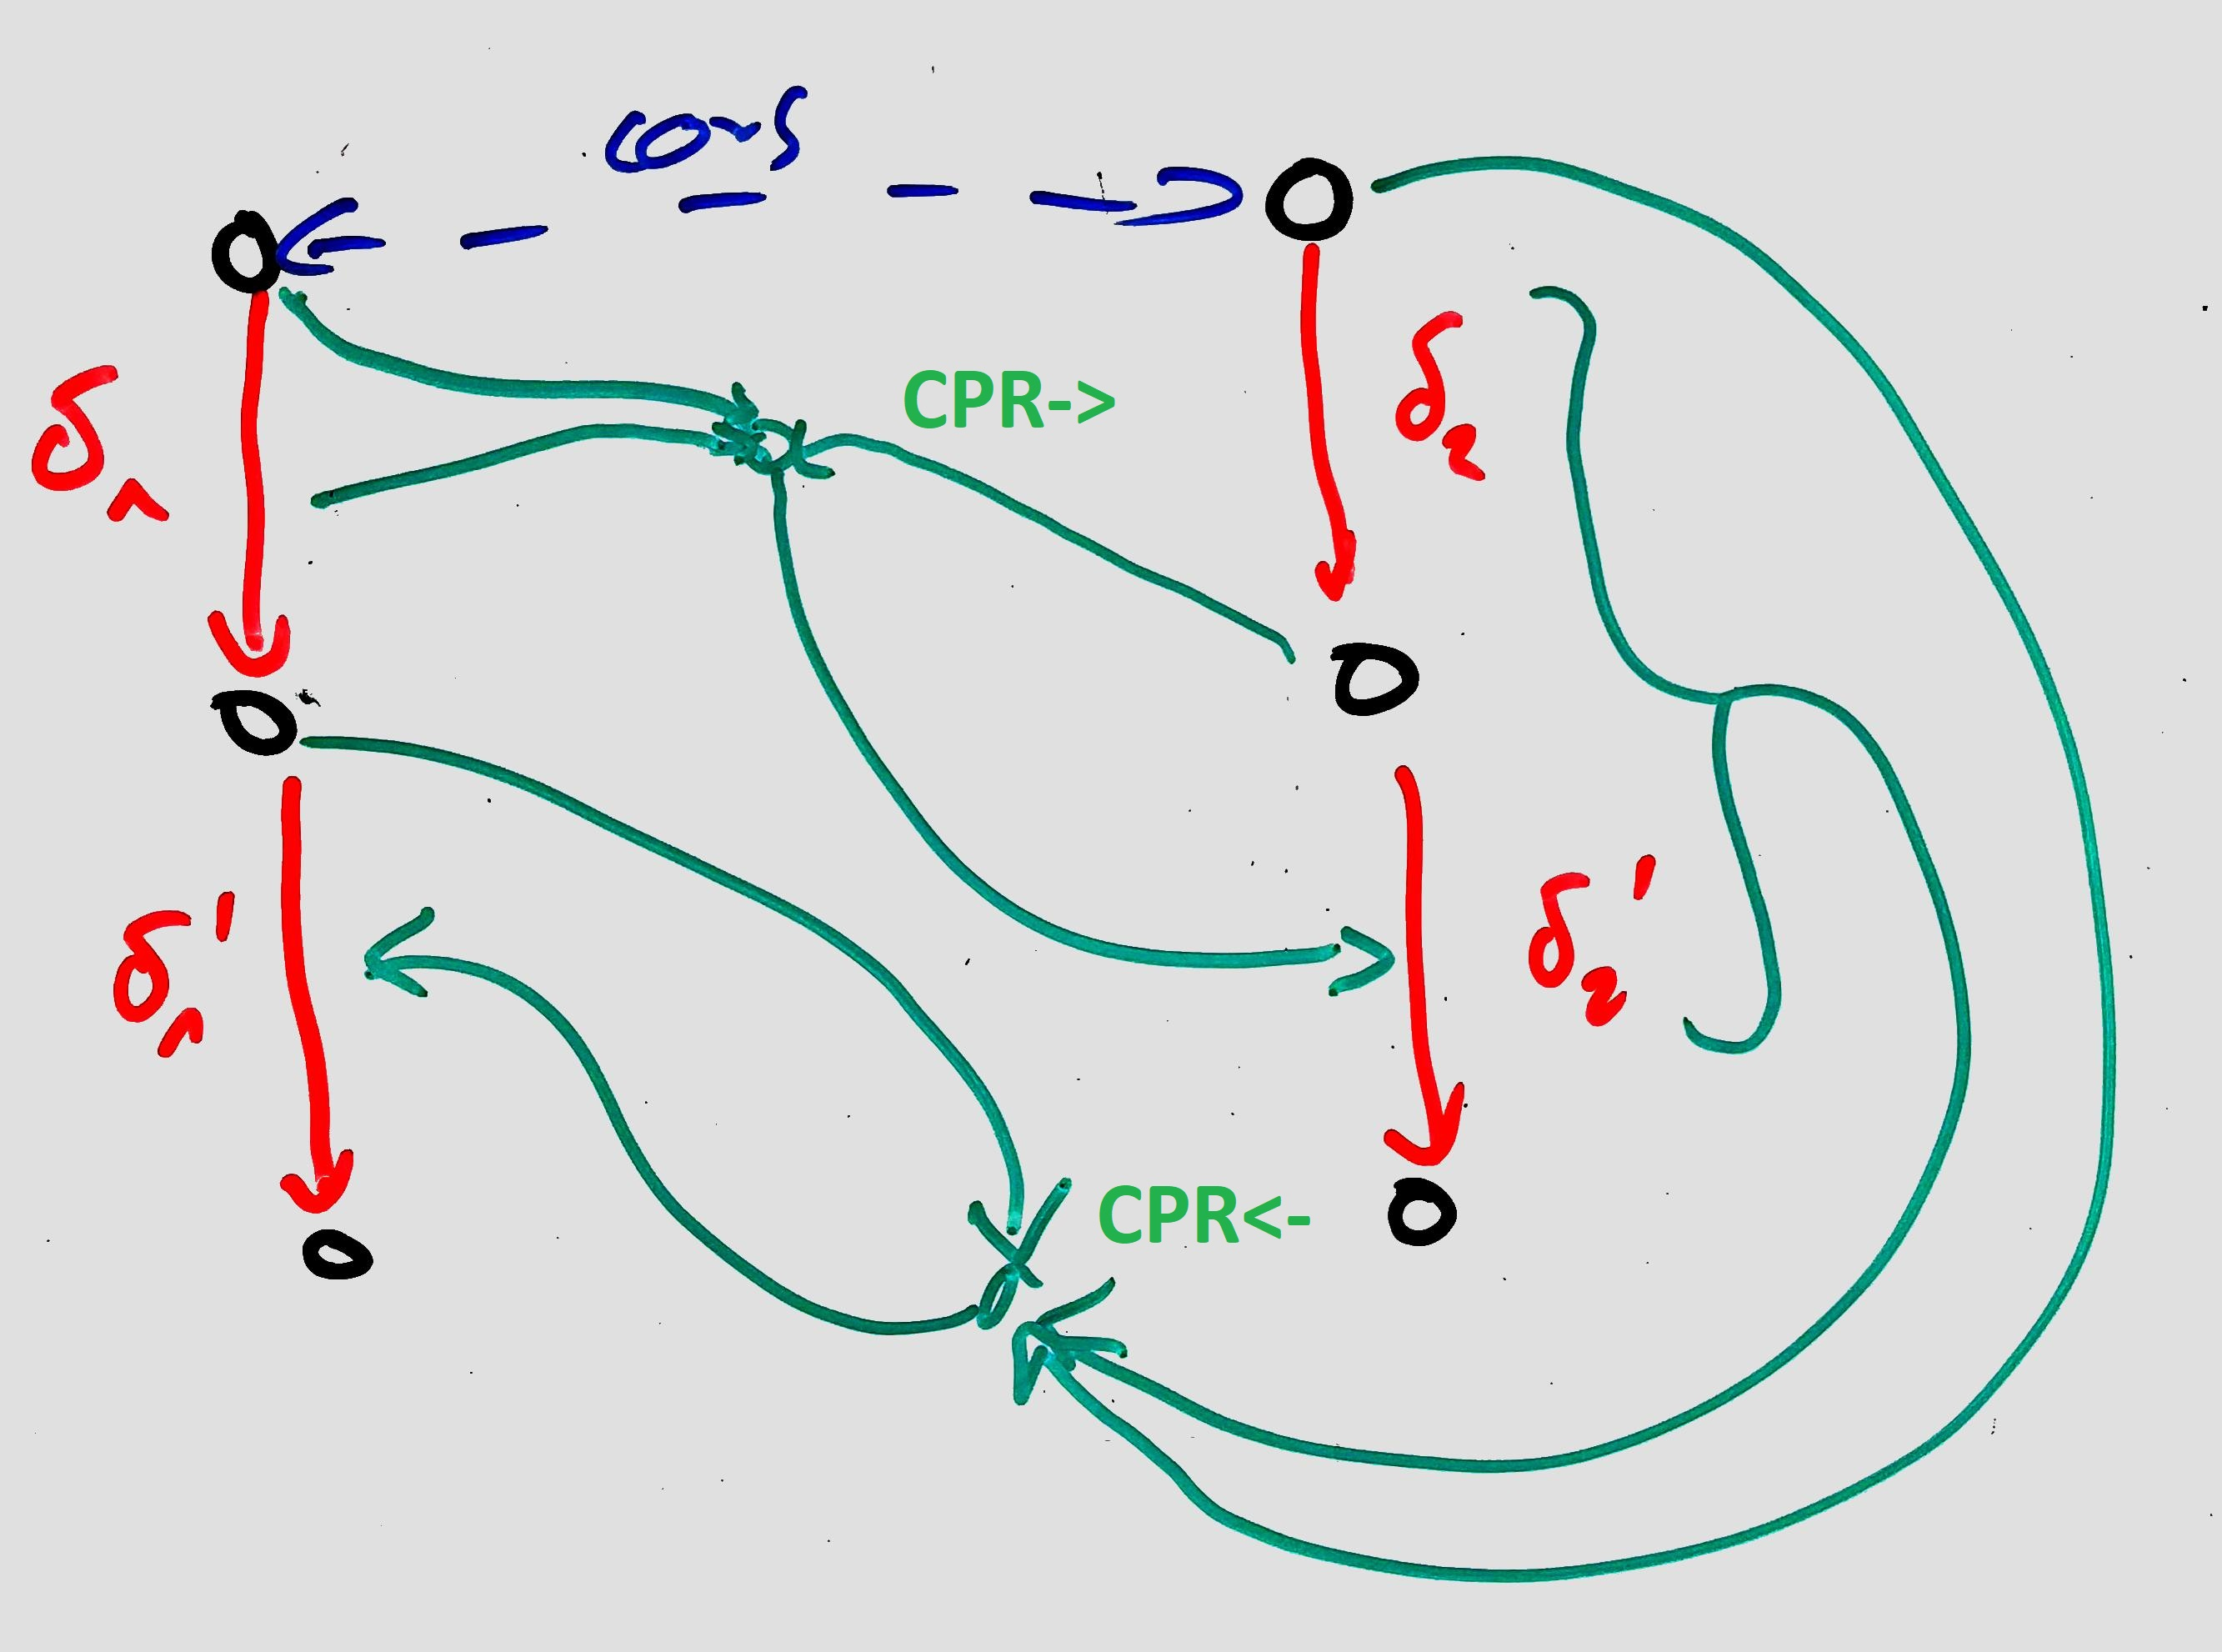
\includegraphics[width=0.7\textwidth]{figures/correctness/synchronization/synchronizing_execution_step.jpg}    
    \caption[Synchronizing bidirectional transformation execution step]{Operation of a synchronizing bidirectional transformation execution step.}
    \label{fig:synchronization:synchronizing_execution_step}
\end{figure}

\mnote{Execute step of a transformation to integrate changes to both models}
Since we want consider the case that both of the models instead of only one of them have been modified, we extend the approach to process changes to both models.
More precisely, we introduce a modified notion of transformation execution steps, which is able to process changes to both models.
The operation of that execution step is depicted in \autoref{fig:synchronization:synchronizing_execution_step}.
To this end, the first executed consistency preservation rule is applied to the first model and the change to it, but receives the modified state of the second model.
We have motivated the necessity not to apply the first consistency preservation rule to the unmodified second model in \autoref{chap:synchronization:combination:sequencing}.
Afterwards, we apply the second consistency preservation rule to the unmodified first model and introduce the modifications to the second model as the concatenation of the original change and the one introduced by the first consistency preservation rule.
This way, we ensure that all inconsistencies are introduced by changes that are processed by the consistency preservation rules, which was our requirement for practical applicability due to the necessity only to react to changes instead of processing arbitrarily inconsistent models states.

\begin{definition}[Synchronizing Bidirectional Transformation Execution Step]
    \label{def:synchronizingtransformationexecutionstep}
    Let $\transformation{t} = \tupled{\consistencyrelationset{CR}, \consistencypreservationrule{\consistencyrelationset{CR}}^{\rightarrow}, \consistencypreservationrule{\consistencyrelationset{CR}}^{\leftarrow}}$ be a bidirectional transformation for metamodels $\metamodel{M}{1}$ and $\metamodel{M}{2}$.
    A \emph{synchronizing execution step} $\function{SyncEx}_{\transformation{t}}^1$ of $\transformation{t}$ is a function:
    \begin{align*}
        \function{SyncEx}_{\transformation{t}}^1 : \; & (\metamodelinstanceset{M}{1}, \metamodelinstanceset{M}{2}, \changeuniverse{\metamodel{M}{1}}, \changeuniverse{\metamodel{M}{2}}) \rightarrow (\metamodelinstanceset{M}{1}, \metamodelinstanceset{M}{2}, \changeuniverse{\metamodel{M}{1}}) \cup \setted{\bot} \\
        & (\model{m}{1}, \model{m}{2}, \change{\metamodel{M}{1}}, \change{\metamodel{M}{2}}) \mapsto 
        \begin{cases} 
            (\model{m}{1}', \model{m}{2}', \change{\metamodel{M}{1}}') \\
            \bot
        \end{cases}
    \end{align*}
    with:
    \begin{align*}
        & \change{\metamodel{M}{2}}' = \consistencypreservationrule{\consistencyrelationset{CR}}^{\rightarrow}(\model{m}{1}, \change{\metamodel{M}{2}}(\model{m}{2}), \change{\metamodel{M}{1}}) %\\
        & \model{m}{1}' = \change{\metamodel{M}{1}}(\model{m}{1}) \\
        & \change{\metamodel{M}{1}}' = \consistencypreservationrule{\consistencyrelationset{CR}}^{\leftarrow}(\model{m}{2}, \model{m}{1}', \change{\metamodel{M}{2}}' \concatfunction \change{\metamodel{M}{2}}) %\\
        & \model{m}{2}' = \change{\metamodel{M}{2}}'(\change{\metamodel{M}{2}}(\model{m}{2}))
    \end{align*}
    If either consistency preservation rule is undefined for the input, i.e., $\consistencypreservationrule{\consistencyrelationset{CR}}^{\rightarrow}(\model{m}{1}, \change{\metamodel{M}{2}}(\model{m}{2}), \change{\metamodel{M}{1}}) = \bot$ or $\consistencypreservationrule{\consistencyrelationset{CR}}^{\leftarrow}(\model{m}{2}, \model{m}{1}', \change{\metamodel{M}{2}}' \concatfunction \change{\metamodel{M}{2}}) \bot$, then the execution is undefined, i.e., $\function{SyncEx}_{\transformation{t}}^1(\model{m}{1}, \model{m}{2}, \change{\metamodel{M}{1}}) = \bot$.
    % for given models $\model{m}{1} \in \metamodelinstanceset{M}{1}$, $\model{m}{2} \in \metamodelinstanceset{M}{2}$ and a change $\change{\metamodel{M}{1}} \in \changeuniverse{\metamodel{M}{1}}$ to $\model{m}{1}$ is the consecutive execution of $\consistencypreservationrule{\consistencyrelationset{CR}}^{\rightarrow}$ and $\consistencypreservationrule{\consistencyrelationset{CR}}^{\leftarrow}}$, i.e.
    % \begin{align*}
    %     & \change{\metamodel{M}{2}}' = \consistencypreservationrule{\consistencyrelationset{CR}}^{\rightarrow}(\model{m}{1}, \model{m}{2}, \change{\metamodel{M}{1}}) \\
    %     & \change{\metamodel{M}{1}}' = \consistencypreservationrule{\consistencyrelationset{CR}}^{\leftarrow}(\model{m}{2}, \change{\metamodel{M}{1}}(\model{m}{1}), \change{\metamodel{M}{2}}')
    % \end{align*}
    % with the resulting changes $\change{\metamodel{M}{1}}'$ and $\change{\metamodel{M}{2}}'$.
\end{definition}

\mnote{Synchronization step needs to be executed only once}
The synchronizing bidirectional execution step is necessary to first integrate the changes made in both models.
It is defined such that it only produces a change in the first model, such that afterwards ordinary transformation execution steps that only need to deal with a change to one model have to be applied.
This leads the \autoref{algo:synchronization:executesynchronizingbidirectionaltransformation} for the execution of a synchronizing bidirectional transformation.
%Step integrates both changes, comparable to ordinary step, but first treats changes to m2 as already applied, i.e., given models are inconsistent, then processes the changes in the opposite direction to generate necessary changes to restore consistency from them.

\begin{algorithm}
    \begin{algorithmic}[1]
    \Procedure{\function{ExecuteSync}}{$\transformation{t} = \tupled{\consistencyrelationset{CR}, \consistencypreservationrule{\consistencyrelationset{CR}}^{\rightarrow}, \consistencypreservationrule{\consistencyrelationset{CR}}^{\leftarrow}}, \model{m}{1}, \model{m}{2}, \change{\metamodel{M}{1}}, \change{\metamodel{M}{2}}$}
        \algindentskip
        \If{$\neg (\tupled{\model{m}{1}, \model{m}{2}} \consistenttomath \consistencyrelationset{CR})$}
            \State \Return{$\bot$}
        \EndIf
        \algblockskip

        \If{$\neg (\tupled{\change{\metamodel{M}{1}}(\model{m}{1}), \model{m}{2}} \consistenttomath \consistencyrelationset{CR})$} \label{algo:synchronization:execute_synchronizing_bidirectional_transformation:line:synchronizationstart}
            \State $executionResult$ $\leftarrow$ $\function{SyncEx}_\transformation{t}^1(\model{m}{1}, \model{m}{2}, \change{\metamodel{M}{1}}, \change{\metamodel{M}{2}})$
            \If{$executionResult = \bot$}
                \State \Return{$\bot$} \label{algo:synchronization:execute_synchronizing_bidirectional_transformation:line:returnbot1}
            \Else
                \State $(\model{m}{1}, \model{m}{2}, \change{\metamodel{M}{1}}) \gets executionResult$
            \EndIf
        \EndIf \label{algo:synchronization:execute_synchronizing_bidirectional_transformation:line:synchronizationend}
        \algblockskip

        \While{$\neg (\tupled{\change{\metamodel{M}{1}}(\model{m}{1}), \model{m}{2}} \consistenttomath \consistencyrelationset{CR})$}
            \State $executionResult$ $\leftarrow$ $\function{Ex}_\transformation{t}^1(\model{m}{1}, \model{m}{2}, \change{\metamodel{M}{1}})$
            \If{$executionResult = \bot$}
                \State \Return{$\bot$} \label{algo:execute_synchronizing_bidirectional_transformation:line:returnbot2}
            \Else
                \State $(\model{m}{1}, \model{m}{2}, \change{\metamodel{M}{1}}) \gets executionResult$
            \EndIf
        \EndWhile
        \algblockskip

        \State \Return{$\tupled{\change{\metamodel{M}{1}}(\model{m}{1}), \model{m}{2}}$} \label{algo:synchronization:execute_synchronizing_bidirectional_transformation:line:returnresult}
        \algindentskip
    \EndProcedure
\end{algorithmic}
    \caption[Execution of a bidirectional transformation for synchronization]{Execution of a bidirectional transformation in the synchronization case.}
    \label{algo:synchronization:executesynchronizingbidirectionaltransformation}
\end{algorithm}

\mnote{Synchronizing transformation execution has same properties than non-synchronizing one}
This algorithm has the same properties as the one for the non-synchronization case given in \autoref{algo:synchronization:executebidirectionaltransformation}.
It does always terminate and either returns $\bot$ or a consistent pair of models.

\begin{theorem}[Consistent Termination of Partial-Consistency-Improving Synchronizing Bidirectional Transformation Execution]
    \label{theorem:synchronizingbidirectionaltransformationconsistencytermination}
    Let $\transformation{t} = \tupled{\consistencyrelationset{CR}, \consistencypreservationrule{\consistencyrelationset{CR}}^{\rightarrow}, \consistencypreservationrule{\consistencyrelationset{CR}}^{\leftarrow}}$ be a partial-consistency-improving bidirectional transformation.
    Then \autoref{algo:synchronization:executesynchronizingbidirectionaltransformation} does always terminate and either returns $\bot$ or a consistent model pair.
\end{theorem}
\begin{proof}
    The algorithm is identical to \autoref{algo:synchronization:executebidirectionaltransformation}, except for Lines~\ref{algo:synchronization:executesynchronizingbidirectionaltransformation:line:synchronizationstart}--\ref{algo:synchronization:executesynchronizingbidirectionaltransformation:line:synchronizationend}, which add the initial synchronization step.
    These lines add a single return statement that can return $\bot$.
    Since the return statement not returning $\bot$ is still preceded by the while loop having the loop condition that the model pair needs to be inconsistent, the argument of the proof for \autoref{lemma:bidirectionaltransformationconsistency} regarding non-synchronizing bidirectional transformations ensuring that only consistent models are returned still applies.
    Thus, we know the algorithm either returns $\bot$ or a consistent model pair.

    Termination of the algorithm is guaranteed for the same reasons as for non-synchronizing bidirectional transformations as proven in \autoref{lemma:bidirectionaltransformationtermination}.
    Although the additional execution of $\function{SyncEx}$ may introduce further inconsistencies, the proof already considered that the models given to the while loop may be arbitrarily inconsistent.
    Thus, the inductive improvement in partial consistency through the while loop is given in the same way and thus, finally, the model pair becomes consistent.
\end{proof}

\mnote{Transformation only need to deal with inconsistencies introduced by changes}
Thus, we have proven that we can execute a bidirectional transformation that is partial-consistency-improving for two given models and changes to both of the, such that consistent models are delivered, as long as the transformation is able to process the changes.
In fact, we have already restricted the algorithm such that it must not be able to deal with arbitrarily inconsistent models, but only with models that are initially given, such that only the given changes introduce inconsistencies.
This is supposed to make it easier to define transformation in practice that fulfill the property of being partial-consistency-improving, as they can rely on the assumption that inconsistency is only introduced by the given changes.

\mnote{Definition of synchronizing bidirectional transformations}
With the insight that partial-consistency-improving bidirectional transformations can be used to integrate changes to both of two models and deliver consistent models based on that changes, we can define \emph{synchronizing bidirectional transformations} as bidirectional transformations with the property of being partial-consistency-improving.

\begin{definition}[Synchronizing Bidirectional Transformation]
    Let $\transformation{t}$ be a partial-consistency-improving bidirectional transformation.
    Then we call $\transformation{t}$ a \emph{synchronizing bidirectional transformation}.
\end{definition}

\mnote{Order of consistency preservation rules provides no conceptual benefit but may improve usability}
As we have already discussed at the end of \autoref{chap:synchronization:bidirectional:transformations}, we defined bidirectional transformation execution steps starting with $\consistencypreservationrule{\consistencyrelationset{CR}}^{\rightarrow}$, although it may also be necessary to start with $\consistencypreservationrule{\consistencyrelationset{CR}}^{\leftarrow}$ if a change was performed in the second model.
We discussed that our definitions are without loss of generality and can be directly transferred by swapping the rules.
For the synchronization case, in which both models have been modified, it does, theoretically, not even make a difference which of the consistency preservation rules is executed first, because changes to both models are present anyway.
From a practical perspective, it can, however, make sense to define one the consistency preservation rules as the one to always be executed first.
For example, it might make sense to first execute the consistency preservation rule from the more abstract to the more detailed model, if such a relation exists between the models.
We leave such considerations up to the individual transformation developer or future research, as the selection of the order does not provide any conceptual benefits, but, in the best case, eases the definition of appropriate consistency preservation rules and improves usability.

\todo{Define synchronizing bidirectional transformation as a partial-consistency-improving bidirectional transformation}


\subsection{Equivalence to Synchronizing Transformations}

\mnote{Synchronizing and synchronizing bidirectional transformations have equal inputs and outputs}
For our definition of transformation networks, we used the notion of synchronizing transformations (cf.~\autoref{def:synchronizingtransformation}), whose single consistency preservation rule accept two consistent models and a change to each of them and return two changes that, if applied to the models, result in consistent models again.
Synchronizing bidirectional transformations, i.e., the yet defined transformations, which are composed of two unidirectional consistency preservation rules, also accept two consistent models and a change to each of them and return two consistent models.
We could also define those transformations to return changes rather than the consistent models by simply concatenating all changes calculated by the transformation execution steps.
For reasons of simplicity, we omitted that in the formal description.

\mnote{Synchronizing and synchronizing bidirectional transformations have equal expressiveness}
Although synchronizing transformations and synchronizing bidirectional transformations have the same requirements to their inputs and provide the same guarantees regarding consistency for their output, both may also return $\bot$ to indicate that they were not able to calculate changes that lead to consistent models.
While a synchronizing transformation can be defined such that it never return $\bot$ by defining a consistency preservation rule that is a total function, the possibility of a synchronizing bidirectional transformation to never return $\bot$ depends on the interplay of the two unidirectional consistency preservation rules.
Nevertheless, we can show that both have equal expressiveness, i.e., they can always return the same results for the same inputs.

\begin{theorem}[Synchronizing Bidirectional Transformation Expressiveness]
    Synchronizing bidirectional transformations have equal expressiveness than synchronizing transformations.
\end{theorem}
\begin{proof}
    Each synchronizing bidirectional transformation can be realized by a synchronizing transformation by simply defining the function of the consistency preservation rule such that it returns the result that is produced by the execution of the synchronizing bidirectional transformation.
    Let $\transformation{t}$ be a synchronizing bidirectional transformation with:
    \begin{align*}
        \function{ExecuteSync}(\transformation{t}, \model{m}{1}, \model{m}{2}, \change{\metamodel{M}{2}}) = (\model{m}{1}', \model{m}{2}')
    \end{align*}
    Then we define the consistency preservation rule $\consistencypreservationrule{}$ of a synchronizing transformation as:
    \begin{align*}
        &
        \consistencypreservationrule{}(\model{m}{1}, \model{m}{2}, \change{\metamodel{M}{1}}, \change{\metamodel{M}{2}}) = (\model{m}{1}, \model{m}{2}, \change{\metamodel{M}{1}}', \change{\metamodel{M}{2}}') \\
        & \formulaskip
        \withmath \change{\metamodel{M}{1}}'(\change{\metamodel{M}{1}}(\model{m}{1})) \equivalentperdefinition \model{m}{1}' 
        \land \change{\metamodel{M}{2}}'(\change{\metamodel{M}{2}}(\model{m}{2})) \equivalentperdefinition \model{m}{2}'
    \end{align*}
    Then, per definition, applying the resulting changes to the input models, the synchronizing transformation delivers for every possible input the same result by applying $\consistencypreservationrule{}$ as the synchronizing bidirectional transformation.

    Realizing a synchronizing transformation by a synchronizing bidirectional transformation requires the repeated execution of the two consistency preservation rules to emulate the behavior of the single 
    synchronizing consistency preservation rule.
    Let $\consistencypreservationrule{}$ be the consistency preservation rule of a synchronizing transformation with:
    \begin{align*}
        \consistencypreservationrule{}(\model{m}{1},\model{m}{2},\change{\metamodel{M}{1}},\change{\metamodel{M}{2}}) = (\model{m}{1},\model{m}{2},\change{\metamodel{M}{1}}',\change{\metamodel{M}{2}}')
    \end{align*}
    Then we can define the two unidirectional consistency preservation rules of the synchronizing transformation $\transformation{t}$ as follows.
    \begin{align*}
        & 
        \consistencypreservationrule{}^{\rightarrow}(\model{m}{1},\change{\metamodel{M}{2}}(\model{m}{2}),\change{\metamodel{M}{1}}) = \change{\metamodel{M}{2}}'' \withmath \change{\metamodel{M}{2}}''(\change{\metamodel{M}{2}}(\model{m}{2})) \equivalentperdefinition \change{\metamodel{M}{2}}'(\model{m}{2}) \\
        &
        \consistencypreservationrule{}^{\leftarrow}(\model{m}{2},\change{\metamodel{M}{1}}(\model{m}{1}),\change{\metamodel{M}{2}}'' \concatfunction \change{\metamodel{M}{2}}) = \change{\metamodel{M}{1}}'' \withmath \change{\metamodel{M}{1}}''(\change{\metamodel{M}{1}}(\model{m}{1})) \equivalentperdefinition \change{\metamodel{M}{1}}'(\model{m}{1})
    \end{align*}
    So we simply define the two consistency preservation rules in a way such that each of them delivers for the inputs in the synchronizing execution step $\function{SyncEx}_{\transformation{t}}^1$ according to \autoref{def:synchronizingtransformationexecutionstep} those changes that are necessary to produce exactly the results of the consistency preservation rule $\consistencypreservationrule{}$ of the synchronizing transformation.
    Then according to the behavior of $\function{SyncEx}_{\transformation{t}}^1$, we have:
    \todo{Vielleicht besser Striche über Buchstaben statt noch mehr Apostrophe}
    \begin{align*}
        &
        \function{SyncEx}_{\transformation{t}}^1(\model{m}{1},\model{m}{2},\change{\metamodel{M}{1}},\change{\metamodel{M}{2}}) = (\model{m}{1}'', \model{m}{2}'', \change{\metamodel{M}{1}}''') \withmath \\
        & \formulaskip
        \change{\metamodel{M}{1}}'''(\model{m}{1}'') = % per def SyncEx
        \change{\metamodel{M}{1}}'''(\change{\metamodel{M}{1}}(\model{m}{1})) = % per def SyncEx and per def above
        %\consistencypreservationrule{}^{\leftarrow}(\model{m}{2},\change{\metamodel{M}{1}}(\model{m}{1}),\change{\metamodel{M}{2}}'' \concatfunction \change{\metamodel{M}{2}})(\change{\metamodel{M}{1}}(\model{m}{1})) % per def above
        \change{\metamodel{M}{1}}'(\model{m}{1}) \\
        & \formulaskip
        \land
        \model{m}{2}'' = \change{\metamodel{M}{2}}'(\model{m}{2})
    \end{align*}
    So $\function{SyncEx}_{\transformation{t}}^1$ produces $\model{m}{1}''$, $\model{m}{2}''$ and $\change{\metamodel{M}{1}}'''$ for which we know that $\change{\metamodel{M}{1}}'''(\model{m}{1}'')$ and $\model{m}{2}''$ are consistent, because their equivalents $\change{\metamodel{M}{1}}'(\model{m}{1})$ and $\change{\metamodel{M}{2}}'(\model{m}{2})$ are consistent by assumption.
    Thus, the execution of the synchronizing bidirectional transformation $\transformation{t}$ according to \autoref{algo:synchronization:executesynchronizingbidirectionaltransformation} terminates after the conditional statement in \autoref{algo:synchronization:executesynchronizingbidirectionaltransformation:line:synchronizationstart} with the same consistent models that are delivered by the applying the changes calculated by the consistency preservation rule $\consistencypreservationrule{}$ of the assumed synchronizing transformation.

    With these construction approaches in both directions, we have shown that each synchronizing transformation can be expressed by a synchronizing bidirectional transformation and vice versa.
\end{proof}

\mnote{Executing only one synchronizing execution step will not lead to consistency in pratice}
Although we have proven that each synchronizing transformation can be expressed by a synchronizing bidirectional transformations and thus the latter ones can be used to express any desired consistency preservation in a transformation network, the constructive approach in the proof does not reflect a practical construction approach for the unidirectional consistency preservation rules of a synchronizing bidirectional transformation.
In practice, it will usually not be possible to define the rules in a way that they deliver consistent models after executing each ones, as we already discussed in \autoref{chap:synchronization:combination:bounds}.
It shows, however, that it would possible in theory.

\mnote{Synchronizing bidirectional transformations can be used in transformation networks}
Based on the knowledge that we can use synchronizing bidirectional transformations in transformation networks, we discuss in the following how a transformation developer can actually achieve that the specification of a bidirectional transformation in terms of two unidirectional consistency preservation rules does actually fulfill the requirements of being partial-consistency-improving and thus synchronizing.


% We yet discussed how to integrate one change on partially consistent models.
% Now we apply to this be able to integrate changes to both models.
% Describe the process here:

% Two step process.
% 1 Integrate changes to both models.
% d2' = CPRr(m1, d2(m2), d1) und d1' = CPRl(m2, d1(m1), d2' o d2)
% 2. Iteratively propagate changes.
% d2'' = CPRr(d1(m1), d2' o d2(m2), d1')
% d1'' = CPRl(d2' o d2(m2), d1(m1), d2'')
% etc. 

% The first step is special, because CPRl needs to process both the original changes as well as the ones generated by CPRr in the first step.
% In all further steps it is only necessary to process the changes just generated by the other CPR.

% DISCUSS: Which CPR to execute first? One is the "leading" one. Integrate its changes first. Can be determined by abstraction, or, theoretically, it completely irrelevant. Only a practical consideration.



% \section{Old contents to integrate}

%%
%% THE DIRECTIONALITY GAP: Formal framework considers bidirectional transformations, practically we have unidirectional ones
%%
% \subsection{The Directionality Gap}

% \mnote{Unidirectional synchronizing preservation rules to close the gap}
% To come up with an approach to combine unidirectional consistency preservation rules to behave as a single synchronizing one, we first identify how we can decompose synchronizing consistency preservation rules into unidirectional ones.
% We then relate these unidirectional synchronizing rules to the non-synchronizing ones defined in transformation languages.

% \mnote{Fine-grained consistency relations allow to define relation between unidirectional preservation rules}
% In \autoref{chap:compatibility:formal_notion}, we also discussed that consistency relation can be considered in a fine-grained way that is able to reflect different notion of consistency in both directions of a relation.
% We will base our notion of unidirectional synchronizing rules on those fine-grained relations to be able to find a proper notion of how the rules in both directions are supposed to work together.
% We did, however, also discuss in that chapter that all fine-grained relations can also be translated into \modellevelconsistencyrelations, thus the insights we already had for those model-level relations still apply to the considerations regarding fine-grained ones.

% \mnote{Stick to coarse-grained notion of preservation rules}
% According to the consideration of fine-grained consistency relations, transformation languages also allow the specification of or derive fine-grained consistency preservation rules from a declarative specification.
% They are often called \emph{transformation rules} and composed to a transformation that consists of multiple such rules, each encoding a consistency relations and a preservation rule for it.
% We will, however, stick to the coarse-grained notion of consistency preservation rules, as they are sufficient for our considerations.

% \mnote{New transformation notion based on fine-grained consistency relations}
% In consequence, from now we will consider a synchronizing transformation as a set of fine-grained consistency relations according to \autoref{def:consistencyrelation} and a consistency preservation rule that preserves consistency according to the set of relations.
% The consistency preservation rule and also the complete transformation are thus still considered correct if applying it to a consistent pair of models and changes to them, applying the resulting changes to the models again delivers a pair of models that is consistent to all consistency relations.
% Note that being consistent to all fine-grained consistency relations is equivalent to being consistent to the single \modellevelconsistencyrelation induced by the fine-grained relations.


% \subsubsection{Unidirectional Synchronizing Transformations}

% \mnote{Decomposition of consistency preservation rules into two unidirectional ones}
% To reflect the unidirectional notion of consistency preservation provided by transformation languages in our formalism, we propose a decomposition of consistency preservation rules according to \autoref{def:consistencypreservationrule} into two unidirectional ones.

% \begin{definition}[Unidirectional Consistency Preservation Rule]
%     \label{def:unidirectionalconsistencypreservationrule}
%     Let $\metamodel{M}{1}, \metamodel{M}{2}$ be two metamodels and $\consistencyrelationset{CR}$ a set of consistency relations between elements of those metamodels.
%     A \emph{unidirectional consistency preservation rule} $\consistencypreservationrule{\consistencyrelationset{CR}}$ for the relation set $\consistencyrelationset{CR}$ is a function:
%     \begin{align*}
%         \consistencypreservationrule{\consistencyrelationset{CR}} : (\metamodelinstanceset{M}{1}, \metamodelinstanceset{M}{2}, \changeuniverse{\metamodel{M}{1}}, \changeuniverse{\metamodel{M}{2}}) \rightarrow \changeuniverse{\metamodel{M}{2}}
%     \end{align*}
% \end{definition}

% \mnote{Notation for two related unidirectional rules}
% To be able to explicitly reference the consistency preservation rules for both directions between two metamodels $\metamodel{M}{1}$ and $\metamodel{M}{2}$, we denote the set of consistency relations between $\metamodel{M}{1}$ and $\metamodel{M}{2}$ as $\consistencyrelationset{CR}_{\rightarrow}$ and the one in the opposite direction between $\metamodel{M}{2}$ and $\metamodel{M}{1}$ as $\consistencyrelationset{CR}_{\leftarrow}$.
% We then refer to the two unidirectional consistency preservation rules as:
% \begin{align*}
%     \consistencypreservationrule{\consistencyrelationset{CR}_{\rightarrow}} : (\metamodelinstanceset{M}{1}, \metamodelinstanceset{M}{2}, \changeuniverse{\metamodel{M}{1}}) \rightarrow \changeuniverse{\metamodel{M}{2}}\\
%     \consistencypreservationrule{\consistencyrelationset{CR}_{\leftarrow}} : (\metamodelinstanceset{M}{2}, \metamodelinstanceset{M}{1}, \changeuniverse{\metamodel{M}{2}}) \rightarrow \changeuniverse{\metamodel{M}{1}}
% \end{align*}

% \mnote{Correctness of unidirectional rules analogous to original rules}
% We define correctness of such a unidirectional consistency preservation rule in the same way it was defined for synchronizing consistency preservation rules according to \autoref{def:consistencypreservationrule} and compliant to existing correctness notions for non-synchronizing consistency preservation rules, such as~\cite{stevens2010sosym}.

% \begin{definition}[Unidirectional Consistency Preservation Rule Correctness]
%     \label{def:unidirectionalconsistencypreservationrulecorrectness}
%     Let $\consistencypreservationrule{\consistencyrelationset{CR}}$ be a \emph{unidirectional consistency preservation rule}.
%     We call $\consistencypreservationrule{\consistencyrelationset{CR}}$ \emph{correct} if the resulting models when applying the generated changes are consistent to $\consistencyrelationset{CR}$ again:
%     \begin{align*}
%         &
%         \forall 
%         \model{m}{1} \in \metamodelinstanceset{M}{1}, 
%         \model{m}{2} \in \metamodelinstanceset{M}{2},
%         \change{\metamodel{M}{1}} \in \changeuniverse{\metamodel{M}{1}},
%         \change{\metamodel{M}{2}} \in \changeuniverse{\metamodel{M}{2}} : \\
%         & \formulaskip
%         \tupled{\model{m}{1}, \model{m}{2}} \consistenttomath \consistencyrelationset{CR} \\
%         & \formulaskip
%         \land \exists 
%         \change{\metamodel{M}{2}}' \in \changeuniverse{\metamodel{M}{2}} :
%         \change{\metamodel{M}{2}}' = \consistencypreservationrule{\consistencyrelation{CR}{}}(\model{m}{1}, \model{m}{2}, \change{\metamodel{M}{1}}, \change{\metamodel{M}{2}}) \\
%         & \formulaskip\formulaskip
%         \Rightarrow
%         \tupled{\change{\metamodel{M}{1}}(\model{m}{1}), \change{\metamodel{M}{2}}'(\model{m}{2})} \consistenttomath \consistencyrelationset{CR}
%     \end{align*}
% \end{definition}

% \mnote{Unidirectional synchronizing transformation encapsule a preservation rule for each direction}
% Based on such a unidirectional notion of consistency preservation rule, we can also define a unidirectional notion of transformations, which then consists of two sets of unidirectional consistency relations and two unidirectional consistency preservation rules.

% \begin{definition}[Unidirectional Synchronizing Transformation]
%     \label{def:unidirectionalsynchronizingtransformation}
%     Let $\metamodel{M}{1}$ and $\metamodel{M}{2}$ be two metamodels and $\consistencyrelationset{CR}_{\rightarrow}$ a set of consistency relations between $\metamodel{M}{1}$ and $\metamodel{M}{2}$, as well as $\consistencyrelationset{CR}_{\leftarrow}$ a set of consistency relations between $\metamodel{M}{2}$ and $\metamodel{M}{1}$.
%     Additionally, let $\consistencypreservationrule{\consistencyrelationset{CR}_{\rightarrow}}$ and $\consistencypreservationrule{\consistencyrelationset{CR}_{\leftarrow}}$ be unidirectional consistency preservation rules for both consistency relation sets.
%     A \emph{unidirectional synchronizing transformation} is a quadruple $\transformation{t} = \tupled{\consistencyrelationset{CR}_{\rightarrow}, \consistencyrelationset{CR}_{\leftarrow},\consistencypreservationrule{\consistencyrelationset{CR}_{\rightarrow}}, \consistencypreservationrule{\consistencyrelationset{CR}_{\leftarrow}}}$.
% \end{definition}

% \mnote{Correctness of unidirectional synchronizing transformations}
% We call such a unidirectional synchronizing transformation correct if both consistency preservation rules are correct, i.e., they both preserve consistency according to the underlying consistency relation set.

% \begin{definition}[Unidirectional Synchronizing Transformation Correctness]
%     \label{def:unidirectionalsynchronizingtransformationcorrectness}
%     Let $\transformation{t} = \tupled{\consistencyrelationset{CR}_{\rightarrow}, \consistencyrelationset{CR}_{\leftarrow},\consistencypreservationrule{\consistencyrelationset{CR}_{\rightarrow}}, \consistencypreservationrule{\consistencyrelationset{CR}_{\leftarrow}}}$ be a unidirectional synchronizing transformation.
%     We call $\transformation{t}$ correct if, and only if, $\consistencypreservationrule{\consistencyrelationset{CR}_{\rightarrow}}$ and $\consistencypreservationrule{\consistencyrelationset{CR}_{\leftarrow}}$ are both correct according to \autoref{def:unidirectionalconsistencypreservationrulecorrectness}.
% \end{definition}

% \mnote{Each unidirectional rule only preserves consistency in one direction}
% With a unidirectional synchronizing transformation that adheres to the given correctness definition, we are able to preserve consistency for the consistency relations in each direction between two models.
% Executing either of the unidirectional consistency preservation rules of the transformation does, however, not ensure that the consistency relations for the other direction are fulfilled as well.
% That is the purpose of the other unidirectional consistency preservation rule.

% % \begin{itemize}
%     % \item We assume consistency preservation rules according to fine-grained consistency relations introduced for compatibility
%     % \item So a synchronizing transformation considers fine-grained relations, in fact a transformation then consists of multiple relations, two for each fine-grained relation (each direction). Their combination induces the \modellevelconsistencyrelation for the two metamodels.
%     % \item Although the consistency preservation rule may in practice also be defined in terms fine-grained rules, which together with the fine-grained consistency rules then forms what is often called \emph{transformation rules}, we do not need to have a more fine-grained notion here.
%     % \item The transformation then is still correct as defined before, when the preservation rule preserves consistency to the relation, but now according to all fine-grained relations (and thus also the induced monolithic one) instead to the single model-level one.
%     % \item To reflect the notion of unidirectional consistency preservation rules, as often defined in transformation languages, which are still synchronizing, i.e., are able to react to changes made to both models, we may define:
% % \end{itemize}
% % \begin{align*}
% %     \consistencypreservationrule{\consistencyrelationset{CR}_{\rightarrow},\rightarrow} : (\metamodelinstanceset{M}{1}, \metamodelinstanceset{M}{2}, \changeuniverse{\metamodel{M}{1}}, \changeuniverse{\metamodel{M}{2}}) \rightarrow \changeuniverse{\metamodel{M}{2}})\\
% %     \consistencypreservationrule{\consistencyrelationset{CR}_{\leftarrow},\leftarrow} : (\metamodelinstanceset{M}{1}, \metamodelinstanceset{M}{2}, \changeuniverse{\metamodel{M}{1}}, \changeuniverse{\metamodel{M}{2}}) \rightarrow \changeuniverse{\metamodel{M}{1}})
% % \end{align*}

% \subsubsection{Alignment of Unidirectional Synchronizing Transformations}

% \mnote{Sequential execution of unidirectional rules does not guarantee consistency to relations in both directions}
% It is now possible to execute both consistency preservation rules of a unidirectional synchronizing transformation one after another, as each is able to reflect the changes produced by the other due to the ability to process changes made to both models.
% Thus, we could sequentially calculate:
% \begin{align*}
%     &
%     \change{\metamodel{M}{2}}' = \consistencypreservationrule{\consistencyrelationset{CR}_{\rightarrow}}(\model{m}{1},\model{m}{2},\change{\metamodel{M}{1}},\change{\metamodel{M}{2}})\\
%     &
%     \change{\metamodel{M}{1}}' = \consistencypreservationrule{\consistencyrelationset{CR}_{\leftarrow}}(\model{m}{2},\model{m}{1},\change{\metamodel{M}{2}}',\change{\metamodel{M}{1}})
% \end{align*}
% We then receive the resulting model pair as $\tupled{\change{\metamodel{M}{1}}'(\model{m}{1}), \change{\metamodel{M}{2}}'(\model{m}{2})}$.
% This gives us the guarantee that the resulting model pair is consistent to $\consistencyrelationset{CR}_{\leftarrow}$, as its consistency preservation rule was executed last.
% However, the definitions do not give any guarantee that the model pair is consistent to $\consistencyrelationset{CR}_{\rightarrow}$, as the execution of $\consistencypreservationrule{\consistencyrelationset{CR}_{\leftarrow}}$ may violate some of those relations.

% \mnote{Not violating relations of the other direction is desirable for unidirectional rules}
% It is, however, a desirable property of a unidirectional synchronizing transformation that the consistency preservation rules for the two directions between the same metamodels are aligned with each other in a way that executing the rule in one direction does not lead to further violations of the consistency relations in the other direction.
% This is especially necessary to produce the same behavior as a synchronizing transformation.
% We call such a property \emph{inverse-preserving}, as it ensures that fulfillment of consistency relations of the inverse direction are preserved.

% \begin{definition}[Inverse-Preserving Unidirectional Synchronizing Transformation]%Unidirectional Consistency Preservation Rule}
%     \label{def:inversepreservingunidirectionalsynchronizingtransformation}
%     Let $\transformation{t} = \tupled{\consistencyrelationset{CR}_{\rightarrow}, \consistencyrelationset{CR}_{\leftarrow},\consistencypreservationrule{\consistencyrelationset{CR}_{\rightarrow}}, \consistencypreservationrule{\consistencyrelationset{CR}_{\leftarrow}}}$ be a correct unidirectional synchronizing transformation for two metamodels $\metamodel{M}{1}$ and $\metamodel{M}{2}$.
%     We say that $\transformation{t}$ is \emph{inverse-preserving} if, and only if, executing one of the consistency preservation rules ensures that the resulting models are still consistent to all consistency relations of the opposite direction to which the models were consistent before.
%     For $\consistencypreservationrule{\consistencyrelationset{CR}_{\rightarrow}}$ this is given by the following (for $\consistencypreservationrule{\consistencyrelationset{CR}_{\leftarrow}}$ analogously):
%     \begin{align*}
%         & \forall \model{m}{1} \in \metamodelinstanceset{M}{1}, \model{m}{2} \in \metamodelinstanceset{M}{2}, \change{\metamodel{M}{1}} \in \changeuniverse{\metamodel{M}{1}}, \change{\metamodel{M}{2}} \in \changeuniverse{\metamodel{M}{2}} : \\
%         & 
%         \exists \change{\metamodel{M}{2}}' \in \changeuniverse{\metamodel{M}{2}} : \change{\metamodel{M}{2}}' = \consistencypreservationrule{\consistencyrelationset{CR}_{\rightarrow}}(\model{m}{1},\model{m}{2},\change{\metamodel{M}{1}},\change{\metamodel{M}{2}}) \\
%         & \formulaskip
%         \Rightarrow
%         \forall \consistencyrelation{CR}{} \in \consistencyrelationset{CR}_{\leftarrow}: 
%         \bigl(
%         \tupled{\change{\metamodel{M}{2}}(\model{m}{2}),\change{\metamodel{M}{1}}(\model{m}{1})} \consistenttomath \consistencyrelation{CR}{} \\
%         & \formulaskip\formulaskip
%         \Rightarrow
%         \tupled{\change{\metamodel{M}{2}}'(\model{m}{2}), \change{\metamodel{M}{1}}(\model{m}{1})} \consistenttomath \consistencyrelation{CR}{}
%         \bigr)
%     \end{align*}
% \end{definition}

% \mnote{Inverse-preserving transformations define reasonable alignment}
% This is a reasonable property, because the consistency relations in both directions are usually not disaligned, but only give the freedom to define different consistency notions in both directions, such as more options for consistent elements in one direction than in the other to support different kinds of abstraction.
% It should, however, never be the case that preserving consistency in one direction violates consistency relations in the other direction if transformations are defined properly.

% \mnote{Inverse-preserving transformations can be sequences}
% Given an inverse-preserving unidirectional synchronizing transformation, executing the two unidirectional consistency preservation rules one after another to given consistent models and changes to them preserves consistency to all consistency relations.
% This is a direct consequence of the inverse-preserving property, because no directional rule is allowed to violate consistency that was already ensured in the other direction.

% \begin{theorem}[Inverse-Preserving Unidirectional Synchronizing Transformation Sequencing Correctness]
%     \label{theorem:sequencinginversepreservingtransformations}
%     Let $\transformation{t} = \tupled{\consistencyrelationset{CR}_{\rightarrow}, \consistencyrelationset{CR}_{\leftarrow}, \consistencypreservationrule{\consistencyrelationset{CR}_{\rightarrow}}, \consistencypreservationrule{\consistencyrelationset{CR}_{\leftarrow}}}$ be a correct, inverse-preserving unidirectional synchronizing transformation.
%     Then sequentially executing both consistency preservation rules to given models and changes restores consistency to both consistency relation sets, i.e., given models $\model{m}{1}, \model{m}{2}$ and changes to them $\change{\metamodel{M}{1}}, \change{\metamodel{M}{2}}$, it holds hat:
%     \begin{align*}
%         &
%         \tupled{\model{m}{1}, \model{m}{2}} \consistenttomath \consistencyrelationset{CR}_{\rightarrow}
%         \land \tupled{\model{m}{2}, \model{m}{1}} \consistenttomath \consistencyrelationset{CR}_{\leftarrow}\\
%         &
%         \land \exists \change{\metamodel{M}{2}}' \in \changeuniverse{\metamodel{M}{2}}' : 
%         \change{\metamodel{M}{2}}' = \consistencypreservationrule{\consistencyrelationset{CR}_{\rightarrow}}(\model{m}{1}, \model{m}{2}, \change{\metamodel{M}{1}}, \change{\metamodel{M}{2}}) \\
%         &
%         \land \exists \change{\metamodel{M}{1}}' \in \changeuniverse{\metamodel{M}{1}}' :
%         \change{\metamodel{M}{1}}' = \consistencypreservationrule{\consistencyrelationset{CR}_{\leftarrow}}(\model{m}{2}, \model{m}{1}, \change{\metamodel{M}{2}}', \change{\metamodel{M}{1}}) \\
%         &
%         \Rightarrow \tupled{\change{\metamodel{M}{1}}'(\model{m}{1}), \change{\metamodel{M}{2}}'(\model{m}{2})}\consistenttomath \consistencyrelationset{CR}_{\rightarrow}  \\
%         & \formulaskip
%         \land \tupled{\change{\metamodel{M}{2}}'(\model{m}{2}), \change{\metamodel{M}{1}}'(\model{m}{1})} \consistenttomath \consistencyrelationset{CR}_{\leftarrow}
%     \end{align*}
% \end{theorem}
% \begin{proof}
%     Given models $\model{m}{1}, \model{m}{2}$ that are consistent to $\consistencyrelationset{CR}_{\rightarrow}$ and $\consistencyrelationset{CR}_{\leftarrow}$ and changes $\change{\metamodel{M}{1}}, \change{\metamodel{M}{2}}$, we assume that $\change{\metamodel{M}{1}}'$ and $\change{\metamodel{M}{2}}'$ exist as the results of the consistency preservation rules according to the theorem.
%     If this was not the case, the consistency preservation rules are not defined for the given inputs and thus are not able to produce consistent results, which evaluates the left side of the implication to false, making the whole statement of the theorem true.
%     Now we show correctness of both implied statements:
%     \begin{properenumerate}
%         \item $\tupled{\change{\metamodel{M}{1}}'(\model{m}{1}), \change{\metamodel{M}{2}}'(\model{m}{2})}\consistenttomath \consistencyrelationset{CR}_{\rightarrow}$:
%         As a direction implication of correctness of $\consistencypreservationrule{\consistencyrelationset{CR}_{\rightarrow}}$, we know that $\tupled{\change{\metamodel{M}{1}}(\model{m}{1}), \change{\metamodel{M}{2}}'(\model{m}{2})} \consistenttomath \consistencyrelationset{CR}_{\rightarrow}$.
%         Now the inverse-preserving property of $\transformation{t}$ ensures for the given input of $\consistencypreservationrule{\consistencyrelationset{CR}_{\leftarrow}}$ according to \autoref{def:inversepreservingunidirectionalsynchronizingtransformation} that 
%         \begin{align*}
%         & \forall \consistencyrelation{CR}{} \in \consistencyrelationset{CR}_{\rightarrow}: 
%         \bigl(
%         \tupled{\change{\metamodel{M}{1}}(\model{m}{1}),\change{\metamodel{M}{2}}'(\model{m}{2})} \consistenttomath \consistencyrelation{CR}{} \\
%         & \formulaskip\formulaskip
%         \Rightarrow
%         \tupled{\change{\metamodel{M}{1}}'(\model{m}{2}), \change{\metamodel{M}{2}}'(\model{m}{1})} \consistenttomath \consistencyrelation{CR}{}
%         \bigr)
%         \end{align*}
%         Since the left side of the implication is true for all consistency relations in $\consistencyrelationset{CR}_{\rightarrow}$ due to correctness of $\consistencypreservationrule{\consistencyrelationset{CR}_{\rightarrow}}$, the right side is also true for all consistency relations in $\consistencyrelationset{CR}_{\rightarrow}$.
%         In consequence, we know that $\tupled{\change{\metamodel{M}{1}}'(\model{m}{1}), \change{\metamodel{M}{2}}'(\model{m}{2})} \consistenttomath \consistencyrelationset{CR}_{\rightarrow}$
%         \item $\tupled{\change{\metamodel{M}{2}}'(\model{m}{2}), \change{\metamodel{M}{1}}'(\model{m}{1})} \consistenttomath \consistencyrelationset{CR}_{\leftarrow}$:
%         This directly follows from correctness of $\consistencypreservationrule{\consistencyrelationset{CR}_{\leftarrow}}$.
%     \end{properenumerate}
%     In consequence, sequentially applying both consistency preservation rules of an inverse-preserving unidirectional synchronizing transformation ensures consistency to the consistency relations in both directions.
% \end{proof}

% \mnote{Inverse-preserving unidirectional transformation can emulate synchronizing ones}
% As a consequence of the theorem, we know that we can emulate a synchronizing transformation according to \autoref{def:synchronizingtransformation} with an inverse-preserving unidirectional synchronizing transformation according to \autoref{def:inversepreservingunidirectionalsynchronizingtransformation}.
% We can execute the unidirectional consistency preservation rules one after another to achieve that the resulting models are consistent to all consistency relations in both direction.

% \mnote{Ensuring inverse-preserving property is already a problem of bidirectional transformations}
% In fact, it is not trivial to ensure that two unidirectional transformations are inverse-preserving, even if the consistency relations in both directions are the same, which we will also see in our evaluation of errors in \autoref{chap:errors}.
% This problem, however, already arises when defining bidirectional transformations.
% Transformation languages may derive two unidirectional preservation rules from one specification, so that they are inherently inverse-preserving, or they may allow individual specification of the directions and provide some support for checking that they are aligned with each other, e.g., in the sense that they are inverse-preserving.
% This is, however, an isolated and existing topic of research \todo{Add references for that} and a challenge that already has to be solved for a single bidirectional transformation rather than a network, which is why we do not discuss this problem in more detail here and therefore assume given transformations to be inverse-preserving.

% \mnote{Directionality gap was discussed, synchronization gap remains}
% We have discussed the gap between synchronizing transformations and ordinary transformations defined in transformation languages regarding directionality by decomposing synchronizing transformations into unidirectional ones.
% In the following, we discuss the remaining gap of the formalized transformations being synchronizing, whereas practically defined transformations do not have that property.


%%
%% THE SYNCHRONIZATION GAP: After the directionality gap, we need to discuss how to come from synchronizing to non-synchronizing transformations
%%
% \subsection{The Synchronization Gap}

% \mnote{Practical transformations are not synchronizing}
% Still, there is a gap to practical approaches for defining transformations, as existing approaches do usually not support synchronization, i.e., they are not able to process changes in both models, but only in one of them.
% Transformation languages usually assume that changes are either made by the developer and are then to be propagated to the other model by the transformation, or they are made by the transformation in reaction to changes to the other model.
% The case that developers modify multiple models is sometimes also referred to as a synchronization scenario (although the term is sometimes even used for the simple case of incremental update).
% If we consider that scenario, we will refer to it as \emph{concurrent editing} to avoid confusion.

% \mnote{In contrast to arbitrary concurrent changes, transformation networks produce less conflicts}
% Although the two cases have in common that both instead of only one model involved in a transformation may have been modified, they have a specific difference.
% While user changes to both models can be arbitrarily conflicting, changes performed by other transformations in a network should, in general, not be conflicting, especially if the underlying relations are compatible, as discussed in \autoref{chap:compatibility}.
% For example, if a user changes an element $A$, whose information needs to be propagated to element $B$, but removes element $B$ as well, this cannot be resolved easily, apart from potentially removing element $A$ as well.
% However, as we know from existing approaches for concurrent editing with tools like Git, conflict resolution is not a trivial task~\todo{add cite for difficulty of conflict resolution}.
% Such a scenario may, however, not occur in a transformation network, because if transformations remove elements that are to be updated by others, there will obviously be some conflicts in the transformations manifested in an incompatibility of their consistency relations.

% \mnote{Definition of ordinary transformations}
% An ordinary unidirectional consistency preservation rule as defined in or produced by a transformation language looks as follows:
% \begin{align*}
%     \consistencypreservationrule{\consistencyrelationset{CR}_{\rightarrow}} : (\metamodelinstanceset{M}{1}, \metamodelinstanceset{M}{2}, \changeuniverse{\metamodel{M}{1}}) \rightarrow \changeuniverse{\metamodel{M}{2}}
% \end{align*}
% Such a rule is not synchronizing, i.e., it does not consider that the second model was modified as well, like we defined for unidirectional consistency preservation rules in \autoref{def:unidirectionalconsistencypreservationrule}.

% \mnote{Passing changed models to consistency preservation rule is not possible}
% Given models $\model{m}{1},\model{m}{2}$ and changes $\change{\metamodel{M}{1}},\change{\metamodel{M}{2}}$, if we simply pass the changed model $\model{m}{2}$ to the preservation rule, we call $\consistencypreservationrule{\consistencyrelationset{CR}_{\rightarrow}}(\model{m}{1},\change{\metamodel{M}{2}}(\model{m}{2}),\change{\metamodel{M}{1}})$.
% Then, in general, the behavior of the function is undefined.
% As defined in \autoref{def:consistencypreservationrulecorrectness}, we only required the function to return a change such that applying all changes produces consistent models if the original models were consistent.
% In this case, however, the given models are not necessarily consistent to each other.

% %\subsection{Closing the Gap}
% \mnote{Emulate synchronizing transformations with non-synchronizing ones}
% We thus want to achieve a slight adaptation of those non-synchronizing unidirectional consistency preservation rules, such that they support the case that they support the synchronization case, i.e., that the second model has already been modified.
% Informally speaking, we want to emulate unidirectional synchronizing consistency preservation rules with non-synchronizing ones.
% Additionally, we want to ensure that if such a rule is inverse-preserving for consistent inputs, it is also inverse-preserving for the case that the second model was already modified, such that executing both rules consecutively ensures consistency to the relations in both directions, as we have already proven for inverse-preserving synchronizing transformations in \autoref{theorem:sequencinginversepreservingtransformations}.

% \mnote{Find requirements for non-synchronizing transformations to impose same behavior as synchronizing ones}
% We thus want to find out what has to be considered to define a pair of ordinary, non-synchronizing consistency preservation rules $\consistencypreservationrule{\consistencyrelationset{CR}_{\rightarrow}}$ $\consistencypreservationrule{\consistencyrelationset{CR}_{\leftarrow}}$ to emulate a unidirectional synchronizing transformation.
% This means that $\consistencypreservationrule{\consistencyrelationset{CR}_{\rightarrow}}$ is able to process an input $\tupled{\model{m}{1},\change{\metamodel{M}{2}}\model{m}{2},\change{\metamodel{M}{1}}}$ and return $\change{\metamodel{M}{2}}'$, such that if $\tupled{\model{m}{1},\model{m}{2}}$ is consistent to $\consistencyrelationset{CR}_{\rightarrow}$, then $\tupled{\change{\metamodel{M}{1}}(\model{m}{1}),\change{\metamodel{M}{2}}' \concatfunction \change{\metamodel{M}{2}}(\model{m}{2})}$ is consistent to $\consistencyrelationset{CR}_{\rightarrow}$ as well (and $\consistencypreservationrule{\consistencyrelationset{CR}_{\leftarrow}}$ analogously).
% Additionally, it requires that the transformation induced by the two non-synchronizing consistency preservation rules is inverse-preserving according to \autoref{def:inversepreservingunidirectionalsynchronizingtransformation}, such that sequentially executing them ensures consistency to all consistency relations in both directions.

% \mnote{Ensure correctness and inverse-preserving}
% To achieve that goal, we discuss all possible combinations of changes made to $\model{m}{1}$ and $\model{m}{2}$ that the consistency preservation rules may need to consider.
% We consider the most atomic types of changes that can be performed and ensure that the finding hold for arbitrary change combinations by composition.
% For each combination of changes processed by $\consistencypreservationrule{\consistencyrelationset{CR}_{\rightarrow}}$ , we need to find out the following (for $\consistencypreservationrule{\consistencyrelationset{CR}_{\leftarrow}}$ analogously):
% \begin{enumerate}
%     \item The consistency preservation rule operates correctly, i.e., the result is still consistent to $\consistencyrelationset{CR}_{\rightarrow}$.
%     \item The transformation is inverse-preserving, i.e., no relation in $\consistencyrelationset{CR}_{\leftarrow}$ that was fulfilled before is violated afterwards.
% \end{enumerate}

% \mnote{Case distinction for all change type combinations necessary}
% In the following section, we perform a case distinction for all possible combinations of changes, specifically for EMOF-based models as the most common and general formalism to describe metamodels and models.
% This allows us to derive which combinations of changes are problematic at all and thus have to be explicitly considered when defining ordinary non-synchronizing transformations to be able to properly use them in a transformation network.
% In consequence, it enables transformation developers to construct transformations with ordinary transformation languages that behave like synchronizing transformations required in networks.



% \begin{itemize}
%     \item Define unidirectional consistency preservation rules as above
%     \item Define correctness of unidirectional consistency preservation rules
%     \item Say that we want to investigate what happens when we apply CPR to m1, d(m2) with m1, m2 consistent instead of to m1, m2
% \end{itemize}

% Define ordinary transformations to take deltas in model 1 and produce deltas in model 2
% Say that unidirectional synchronizing transformations take deltas in both models and update the deltas in one of them.
% Refer to fine-grained formalization regarding compatibility, where consistency relations are directional, thus each directional preservation rule preserves consistency according to the consistency relations in one direction.
% Having synchronizing unidirectional transformation, executing both preserves consistency to both unidirectional consistency relations. However, their must be some kind of conformance of the unidirectional transformation to each other (define how this conformance looks like!), so that executing each once does not lead to violations in the other direction. In general, that may not be possible. In fact, each unidirectional transformation should consider the unidirectional consistency relations of both directions.

% So:
% Ordinary unidirectional transformation for Rr: m1, m2, d1 -> d2, such that (d1(m1), d2(m2)) consistent to all relations in Rr (Rl respectively)
% Synchronizing unidirectional transformation: m1, m2, d1, d2 -> d2', such that (d1(m1), d2'(m2)) consistent to all relations Rr and consistent to all relations in Rl to which is was consistent before (thus no violation of further consistency relations)

% Direct consequence: Executing one transformation after the other ensures that models are consistent to alle relations in Rr and relation

% Based on that, we derive how we can use languages that take deltas in model 1 and produce them in model 2 to emulate synchronizing unidirectional transformations that are able to manage deltas in both models and produce deltas in one of them.
% For that, we make the case distinction and derive the creation pattern.
% For each change merge case, we consider that we somehow "merge" the changes. In general, the change of the transformation to m2 will overwrite the previous change to m2. Then we consider that there is another consistency relation affected by the new change. We show whether/why not the other consistency relation can be violated by that change and discuss how to avoid that.

